%------------------------------------------------------------------------
\chapter{3D Model of Object Context}
\label{3DModelofObjectContext.ch}
%------------------------------------------------------------------------
%revised 21-02-13
% \section{An example Scenario}
% \label{Scenario.sec}
% Point-clouds get captured
% Apply the models on the pointclouds
% By matches for models that are found, we know what object classes should be expected in that place
% Based on this result and the ground truth for each place category, the probability of belonging the place to each category is estimated.

% In this scenario, a situation is considered where a mobile robot wants to look around in a building and make a map including 
% semantic information about the places that it meets in the map. 
% The robot builds a 3D map of the building using, for instance, a SLAM application. 
% Employing the context models, which has been trained for different key object classes, the robot can estimate which object 
% classes are probable to be found in each place that is present in the map. 
% 
% By key objects we are referring to distinctive objects for a place category. These specific object classes should be chosen based on 
% a ground truth which is defined in advance for a place category. It is discussed in Chapter ~\ref{UsingObjectContextforPlaceClassification.ch}
% in more detail.
% 
% Then using the results, showing which object classes are expected in a place and based on the ground truth, for key objects of each place
% category, the place is classified. 

% But for the building of the model it self. the same steps mentioned above for capturing the point cloud would be performed,
% on the pre processed captured point cloud of a place using the annotation tool we have developed, key objects for that 
% specific place category would be annotated. Feature extraction would be run on this annotated point cloud giving training 
% samples. Train samples would be combined from several different pointclouds for the same place category but different 
% instances, Resulting data set would be divided into train, validation and test sets. Using SVM with two kernels the model would be 
% trained.
% 
% More details would be presented in section ~\ref{Implementation.sec}

In this chapter, we define our proposed method and the features used to model the Object Contexts. We also discuss the implementation, obtaining train and test datasets, data annotation, and expected results in detail. Nevertheless, first, let us take a look at some of the challenges we had.

% Moved from Chapter 2 on April 21, 2021
\section{Challenges}
\label{Challenges.sec}

There are challenges regarding modeling the object context that follows:

\begin{itemize}

 \item Train set quality: There could be situations and scenes which are completely different from what has been considered in the train set to build the context model. The closer to an all-encompassing dataset we can get, the more accurate model we can have. This would be a challenge in most projects that involve learning.
	
 \item Annotation of objects in Training data: An easy and reliable tool was needed to annotate 3D objects in pointclouds.
	
 \item Pointcloud quality: The quality of pointclouds is a critical issue. The amount of smoothness in the pointcloud and missing points have a 
 significant effect on the extracted features, which are used to describe surfaces, and as a result, on the context model. 
 Upon capturing pointclouds, due to the sensor's viewpoints or obstacles in its line of sight, the resulting pointcloud might miss some essential points. As a result, the extracted geometry from such surfaces is not accurate (and in some cases, it is wrong).
 
 \item Significant difference in the number of positive samples (feature vectors extracted from a region with annotated object presence) against negative ones in feature vectors extracted from training pointclouds.
 
\end{itemize}


\section{2D vs 3D context, benefits of 3D}
The popularity of devices such as Microsoft Kinect has made 3D data widely accessible. 
Therefore, many researchers and academics have shown tremendous desire to use 3D information in their researches, 
which gives a lot more information about our surroundings compared to 2D data. 
Using 3D data has made it simple to capture geometrical information in addition to visual properties. 
From the output of this type of sensors, we can quickly and directly have access to depth information and 3D 
coordinates of any points that are perceived.

Geometrical features, which are obtained from 3D information, enhance the performance of systems significantly in tasks like feature 
based object detection compared to relying only on visual information. 
Notably, in the problem we are dealing with, building a model for object context, depending on features that only encode changes in intensity and color is not enough. The geometry of surfaces needed to be analyzed, and 3D information facilitates and improves this analysis.



\section{Methodology}
\label{Implementation.sec}

In this section, the procedure of building the context model and how it is applied is described in detail. 
The input in this procedure is the pointcloud of a scene and the output is a list of probability values assigned to all regions in
the scene which corresponds to their likelihood of being the context of a particular object class. 


The input cloud is first preprocessed and then annotated with instances of the object class whose context model is being built. 
Feature extraction runs on this annotated pointcloud and outputs the training samples. Train samples are combined from several different pointclouds for the same object class to make the train set. 
Then the train set is given to the SVM classifier to make the context model. A block diagram in figure ~\ref{SystemOverview.figure} shows 
the system overview.

\begin{figure}[t]
  \centerpsw{SystemOverview}{0.8\columnwidth}
  \caption[System Overview]
  {The overview of the system. Box on the left side shows the Train part of the system while the one on the right shows the prediction part.}
  \label{SystemOverview.figure}
\end{figure}

In the following subsection, we introduce the features used in this work and description of the modules of the system 
will come next.

% Features used
We used PCL ~\cite{Rusu_ICRA2011_PCL} for pointcloud processing and Microsoft Kinect with OpenNi driver to capture these pointclouds.
%In this data type 3D coordinates and color information of a point is saved in a record and then an array of these records forms 
%the pointcloud.

\subsection{Defining some used terms}

Here are some terms that are used through the rest of the text:\\
\\
\textbf{\textit{Point of Interest}}: A point from a pointcloud for or around which analysis is being done.\\
\\
\textbf{\textit{Blob}}: A subset of the pointcloud within a radius $r$ around a point of interest.\\
\\
\textbf{\textit{Query blob}}: The blub from which we are extracting the features.\\
\\
\textbf{\textit{QPoint}}: The Query Point that is the center of the query blob.\\
\\
\textbf{\textit{Keypoint}}: All points in downsampled version of an input pointcloud is called {\it Keypoint}. QPoints are selected from keypoints in {\it FeatureExtract} module.\\
\\
\textbf{\textit{OPoint}}: The Object point; is a point in the vicinity of the Qpoint, which is a candidate to be an object point in a positive sample.\\
\\
\textbf{\textit{B-Radius}}: Radius of the sphere around {\it QPoint}. Points that are included in this sphere make the {\it Query blob}.\\
\\
\textbf{\textit{S-Radius}}: Search Radius; is the radius around the {\it QPoint}, within which candidate {\it OPoints} are considered.\\
\\
\textbf{\textit{OPoint-Radius}}: To extract samples from an annotated pointcloud to make a train dataset, for each considered {\it OPoint}, the algorithm look for labeled object point within a small vicinity around it. The radius for this search vicinity is called {\it OPoint-Radius}. If the considered {\it OPoint} is located on an annotated object, there should be a labeled object point very close to it.\\ 
\\
\textbf{\textit{TFP pointcloud}}: Template Full Point pointcloud; is an artificially generated set of point coordinates in the pointcloud format (3D Matrix of points) to be used as candidate viewpoints. It makes a dense cubical pointcloud where its density is based on the selected voxel size. The dimensions of TFP pointcloud get set in a way that it can cover the entire pointcloud from which we want to extract features (for train or test).\\
\\
\textbf{\textit{Voxel-Radius}}: This parameter determines the size of the voxel in TFP pointcloud. its the distance between adjacent points in each dimension.\\
\\
\textbf{\textit{Search blob}}: A subset of {\it TFP pointcloud} within {\it S-Radius} of a {\it QPoint}. 
\\

See figure \ref{FEStructure.figure} and \ref{PointParameters_Diagram.figure}.

\begin{figure}[t]
  \centerpsw{FEStructure2}{0.9\columnwidth}
  \caption[Illustration of the items used in Feature Extract.]
  {Structure used in Feature extraction; The red point is the QPoint; The sphere surrounding it, is the Query Blob; The yellow
  points are some of the OPoint (Best viewed in color).}
  \label{FEStructure.figure}
\end{figure}



\subsection{Object context descriptor}
\label{OCD.ssec}
 
The feature descriptor we proposed in this work consists of the following elements:\\
\\
{\bf local surface orientation}:\\
This element captures a rough estimation of query surface orientation with respect to the vector of gravity. This feature is computed by estimating the angle between the average normal of the surface and the gravity vector. We consider a unit vector along the z-axis in the world coordinate system as the gravity vector. It is noticeable that the position and orientation of the camera with respect to this coordinate system is known and used as
the ground truth to transform pointcloud from Camera coordinate system.\\
\\
{\bf Local surface height}:\\
This element is the average height of the query surface from which the features are extracted with respect to the floor. The floor is assumed to have the lowest height or vertical position in the pointcloud.\\
\\
{\bf Viewpoint Feature Histogram}:\\
This element of the feature vector is a histogram that encodes the geometry of the blob with respect to a specific viewpoint. We found this descriptor very useful for encoding geometry of surfaces in pointclouds for specific viewpoints. The innovative way we took advantage of this powerful descriptor helped us to encode the geometry of surfaces from several different points of view to make our context model independent from the viewpoint. As it was mentioned in \ref{RelatedWork.sec}, being dependant to the viewpoint was a challenge in \cite{aydemir2012_3Dcontext}.
This descriptor is called VFH (~\cite{5651280}), which is explained more in the following subsection. \footnote{The images and definitions are taken from Point Cloud's official website.}

\subsubsection*{The Viewpoint Feature Histogram (VFH)}
\label{VFH.ssec}
 

VFH consists of two components (~\cite{VFH_Definition} and ~\cite{5651280}):


\begin{itemize}
 \item A histogram for viewpoints(128 bins)
 \item A histogram that encodes local geometry(180 bins)
\end{itemize}

The viewpoint component is computed as a histogram of the angles that the direction of the viewpoint  makes with each surface
normals (Figure \ref{VFH_ViewPoint_component.figure}). So for a query blob $S_q$ if we call the viewpoint as $V_p$, for all points of the blub $p_i$ and the surface normal at that point $n_i$ we have $\alpha$ as the angle between $V$ and $n_i$ where $V = V_p - p_i$.

% \begin{equation}
%  \label{VFH_viewpoint.eq}
%     \alpha = angle between (V_p -p_i) , n_i 
% \end{equation}

It is crucial to notice that these angles are between the central direction of the viewpoint and the normal, not each normal's view angle. This is why these features are scale-invariant.  

\begin{figure}[t]
  \centerpsw{ViewPoint_component}{0.8\columnwidth}
  \caption[Viewpoint Component of VFH]
  {Viewpoint part of the feature vector.\cite{VFH_Definition}}
  \label{VFH_ViewPoint_component.figure}
\end{figure}

The second component collects the relative pan, tilt and yaw angles between the direction of 
the surface normal at the centroid of a query blob and the surface normals at other points in the blob.
So for each query blob, the mean curvature around its central point is encoded using a multidimensional histogram of values. If $C$ is the center of the query blub and $p_i$ is one of {\it k-nearest neighbors} of the centroid and $n_i$ is the surface normal at $p_i$, we have three angles and a distance to be captured in this histogram. $\alpha,\theta, \phi$ and $d$, where the angles are pan, tilt and yaw between each pair of normals and $d$ is the distance between $p_i$ and $C$.  


\begin{equation}
 \label{VFH_geometry.eq}
    u = n_C
\end{equation}

\begin{equation}
 V = (p_i -C) \times u
\end{equation}

\begin{equation}
 W = u \times V
\end{equation}

    
Figure  ~\ref{FPFH.figure} Shows the encoded elements and their relations.

% So it consists of accumulated FPFH values for points in the query pointcloud.
%That is the reason why it is referred here \ref{VFH_plot.figure} as extended FPFH.

%FPFH or Fast Point Feature Histogram itself can be considered as a revised version of PFH. FPFH reduces the complexity 
%of PFH algorithm from $ O(n k^{2}) $ to $ O(n k) $ where $n$ is the number of points in the query pointcloud and $k$ is 
%the number of points in the considered neighborhood of each query point. 
%This is the reason why it is called Fast PFH.
%Although it reduces the informativeness of the feature but it would be still enough powerful and impressively faster 
%to compute. 

%PFH captures 3D geometry of the surfaces around a query point and it is invariant to the 6D pose of the query blob's 
%surface. 

%measured for every possible pairs of points in the query point's neighborhood ($ O(n k^{2}) $). 
%In FPFH \cite{FPFH_Definition}, instead of encoding this information for all pairs of points in a neighborhood, It will only 
%take pairs between the query point and its neighbors ($ O(n k) $). 
%At this stage it is referred to as simplified PFH or SPFH. 
%Then to keep the amount of information that this feature can provide, it also estimates SPFH for all $k$ points in the neighborhood.
%The resulting values are integrated with a normalization to result in the FPFH of the query point(equation ~\ref{FPFH.eq}).
% \begin{equation}
%  \label{FPFH.eq}
%  FPFH(P_{q}) = SPFH(P_{q}) + \frac{1}{k} \sum_{i=1}^k {\frac{1}{\omega_k}} \cdot SPFH(k)
% \end{equation}
VFH is robust to different sampling densities or noise levels in the neighborhood of the query point. 
The descriptor is computed by estimating a histogram with concatenated 45 bins for the four different elements mentioned above.

\begin{figure}[t]
  \centerpsw{fpfh_component}{0.65\columnwidth}
  \caption[Local geometry elements of VFH.]
  {Three angles and a distance encoded in the descriptor.\cite{VFH_Definition}}
  \label{FPFH.figure}
\end{figure}

The histogram in this component has 180 bins (4*45 bin).
By adding the viewpoint component (128 bin), it produces a 308 bin histogram.\footnote{We used the available implementation in the Pointcloud Library (PCL)}
The viewpoint component makes the descriptor dependent on the point of view. The viewpoint component is the element that makes a distinction between features captured from a single query blob viewed from different directions.
It is discussed in more detail in Section \ref{FeatureExtract.ssec}.
Despite its dependency on a viewpoint, it still preserves the property of being scale-invariant. 
% Figure ~\ref{VFH_plot.figure} shows a sample plot of VFH and its components.

% \begin{figure}[t]
%   \centerpsw{vfh_histogram}{0.65\columnwidth}
%   \caption[VFH histogram]
%   {A sample plot of VFH and its components.\cite{VFH_Definition}}
%   \label{VFH_plot.figure}
% \end{figure}



The resulting object context descriptor is a vector with 310 elements that encodes a general orientation, height and
geometrical properties of the query blob.
The structure of this descriptor and its elements are shown in Table ~\ref{Descriptor.table}.

\begin{table}
\centering
\caption
[Object context descriptor structure.]
{Structure of object context descriptor.}
\label{Descriptor.table}
\begin{tabular}{|c|c|c|}
\hline
% Field number & 1 & 2 & 3-310 \\
Field number & Content\\

\hline

1 & Orientation\\

\hline

2 & Height\\

\hline

3-130 & Histogram of viewpoints \\

\hline

131-310 &  Histogram of surface angles\\

\hline

\end{tabular}
\end{table}

% Libraries
% \subsection*{Used Libraries in Implementation}
% 
% 


\section{Implementation}

The main implementation is done with C++. Some available libraries are also used in the code, which are listed below.      

\begin{itemize}
 \item {\it PCL} \cite{Rusu_ICRA2011_PCL}
 \item {\it Eigen} \cite{eigenweb}
 \item {\it LIBSVM} \cite{LIBSVM} \& \cite{li2010holistic}
\end{itemize}

Besides the main code, some scripts are written for results evaluation and creating the datasets for experiments in MATLAB. Also, 
scripts creating the experiments and the experimental environment are in python.\\
\\
As illustrated in Figure ~\ref{SystemOverview.figure}, there are five modules in the system:

\begin{itemize}
  \item PreProcess
  \item Annotation
  \item FeatureExtract
  \item Learning
  \item Result visualization
\end{itemize}

\subsection{PreProcess}
\label{PreProcess.ssec}

\begin{figure}[t]
  \centerpsw{PreProcess}{0.9\columnwidth}
  \caption[PreProcess overview]
  {An overview of the PreProcess}
  \label{PreProcessFlowchart.figure}
\end{figure}

 In this module, the input pointclouds get prepared for annotation and feature extraction (see Figure \ref{PreProcessFlowchart.figure}).
 %The pointclouds we used in this work are saved in "PCD" format and their point type is PointXYZRGB which is PCL point type. 
 The processes for capturing these pointclouds are discussed in Section ~\ref{ExperimentalSetup.sec}. 
 
 
 To make all of our calculations consistent and more straightforward, as the first step, we transform the captured pointclouds from the camera coordinate system to the world's coordinate system. Based on the position and orientation of the sensor in time $t_0$, the transformation is done, using the available functions in {\it PCL}.  
 \footnote{Sensor is in a fixed orientation and vertical position in time the first frame is captured for all pointclouds 
 used in experiments of this work.}
 
 
 The essential step in PreProcess, is the estimation of surface normals which is essential for feature extraction. %The accuracy of the VFH feature is directly dependent on the accuracy of the normals. 
 We started with estimating surface normal from each query blob in the feature extract module. However, later we moved to the PreProcess module and estimated the normals for the entire pointcloud once, and saved them in a PCD file to be used whenever needed. During feature extract, estimated normals can be loaded from the file and used to compute features for each query blob. Normals are estimated for each point, using {\it NormalEstimation} class in {\it PCL} which uses PCA method on the covariance matrix of the points.
 
 
 In order to make it easier to classify points, we defined a new point type by adding a field to the original point type ({\it XYZRGB}). This filed is used for labeling each point as {\it object point}, {\it Context point} or {\it others}. The new point type is in {\it XYZRGBL} format, where L is the label field. In case we are modeling contexts for multiple classes of objects, the label can encode all different classes into the points in the pointcloud at the same time. In this step, converting the transformed pointcloud (in the world coordinate system) into XYZRGBL point type is also carried out.
 
 
 There is also one more product for this module, which is discussed more in ~\ref{FeatureExtract.ssec}.
 It is a generated cube-shaped pointcloud with the input cloud's length, width, and height, filled with points. To get the required dimension for this grid pointcloud, we use the 3DMINMAX function from {\it PCL}. A fixed radial distance between them determines the density of these points. It is used as a source for picking viewpoints that are needed in feature extraction.
 
 Therefore, the results of this module are as follows:
 \begin{itemize}
  \item Point-cloud's normals
  \item The transformed version of the input cloud
  \item Converted version
  \item TFP-cloud
 \end{itemize}
 
\begin{algorithm}[t]
\begin{algorithmic}[1]
\REQUIRE Input Point-cloud(XYZRGB).
\REQUIRE Sensor Location and orientation.
\medskip

\STATE Transform the input cloud, based on the Sensor position and orientation from the camera coordinate system to the world coordinate system, and store the result in pointcloud\_Transformed.
\STATE Estimate Normals and store.
\STATE Convert the Pointcloud\_Transformed to Point type XYZRGBL and store in Pointcloud\_Converted.
\STATE Estimate 3DMINMAX of the Pointcloud\_Converted.
\STATE Using the result from the previous step, generate TFP pointcloud.

\medskip
\ENSURE Pointcloud\_Transformed.
\ENSURE Pointcloud\_Normals.
\ENSURE Pointcloud\_Converted(XYZRGBL).
\ENSURE Pointcloud\_Generated(TFP).

\end{algorithmic}
\caption[PreProcess.]
{A brief algorithmic description of PreProcess.}
\label{Preprocess.algorithm}
\end{algorithm}



 
 
\subsection{Annotation}
\label{Annotation.ssec}

\begin{figure}[t]
  \centerpsw{AnnotationFlowchart}{0.9\columnwidth}
  \caption[Annotation overview]
  {An overview of the Annotation}
  \label{AnnotationFlowchart.figure}
\end{figure}


In this module, the transformed and converted version of the pointcloud is loaded and visualized.(see Figure \ref{AnnotationFlowchart.figure}) The visualization is in 3D, and the user can easily manipulate the pointcloud (rotate, zoom in and out, move, etc.) to find the object and select them. 
The objects in the scene can be selected by clicking roughly on their centroid. Once the centroid is selected, the points that are most likely belonging to the same object (within a defined vicinity, closer to each other, compared to points from other adjacent surfaces) get separated and labeled as the points belonging to the object of interest. Labeling the points means assigning the label field (of each of the points) to a value representing a particular object class. 
Objects from different classes get labeled with different values (\ref{Annotation.algorithm}).

\begin{algorithm}[t]
\begin{algorithmic}[1]
\REQUIRE Pointcloud\_Converted(XYZRGBL).
\REQUIRE Object radius(rough estimate).
\medskip

\STATE Visualize input cloud.
\FORALL{objects to be annotated}
  \STATE Run Point picking procedure to get the centroid of an object.
  \STATE Extract closes neighbor points indexes with respect to the input object radius from the vicinity of the picked centroid.
  \STATE Label points whose indexes are extracted in the previous step.
\ENDFOR
\STATE Store the pointcloud with the labels in the output cloud.

\medskip
\ENSURE Pointcloud\_Annotated(XYZRGBL).
\end{algorithmic}
\caption[Annotation.]
{A brief algorithmic description of Annotation.}
\label{Annotation.algorithm}
\end{algorithm}


Figure ~\ref{TrashbinBounding.figure}, shows a scene in an office at {\it Royal Institute of Technology(KTH)}. The object of interest here is the trash bin, which is marked by a green bounding box. This figure is a 2D image of the scene whose pointcloud is available in our dataset, and the annotation is done on the pointcloud.In Figure ~\ref{Annotation.figure} the annotated object could be seen in red within the scene's pointcloud.


It can be seen that some parts of the floor are also colored in red. It means that part of the floor is also annotated as the object. The reason is that the object's radius given to the Annotation tool was not accurate enough, or the center of the object was not picked accurately. However, it does not harm the result, and this much accuracy is more than enough. In similar works, annotation is done using a bounding box (2D or 3D) that considers a box with a specific dimension around the object. The content of that box approximates object points while other points, which do not belong to the object itself, are included. Here, we strictly separate the points of the object by benefiting from the 3D coordinates of the points in the 
pointcloud, so the annotation is more accurate in comparison.


As described in the algorithm ~\ref{Annotation.algorithm}, object segmentation is done automatically in a straightforward way. Based on the picked object center, selecting points from the 3D neighborhood of it separates object points from the 
rest of the pointclouds.

\begin{figure}[t]
  \centerpsw{TrashbinBounding}{0.65\columnwidth}
  \caption[Example scene and object for Annotation tool]
  {An example scene and a trash bin marked by a bounding box as the object which is being annotated (Best viewed in color).}
  \label{TrashbinBounding.figure}
\end{figure}

\begin{figure}[t]
  \centerpsw{Annotation}{0.65\columnwidth}
  \caption[Annotation tool result]
  {An example of annotation result on the pointcloud, red points assumed to belong to the object(Best viewed in color).}
  \label{Annotation.figure}
\end{figure}

We have published this package with its source in GitHub to be used by other researchers and improved by other developers.\cite{AnnotationGithub}


%-----------------------------------------------------------------------------------------------------------------------------
% Feature extraction

\subsection{FeatureExtract}
\label{FeatureExtract.ssec}

\begin{figure}[t]
  \centerpsw{FeatureExtract}{0.9\columnwidth}
  \caption[FeatureExtract overview]
  {An overview of the FeatureExtract process}
  \label{FeatureExtractFlowchart.figure}
\end{figure}


A feature vector, as described in \ref{OCD.ssec}, gets extracted for several pairs of ($QPoint$,$OPoint$) from the entire input pointcloud. 
Figure ~\ref{FEStructure.figure} shows an example for {\it QPoint}, {\it Query blob} and {\it OPoint} for the scene, we saw in Figure 
 ~\ref{TrashbinBounding.figure}. The red point in the figure shows the {\it Query Point}, which is a point from the downsampled version of the same pointcloud. The sphere shown around the {\it QPoint} is the {\it Query blob}. The yellow point is the {\it OPoint} or candidate object point, which in this example is sitting on the annotated object (Trash bin). Therefore it is an object point. In this figure, only some of the {\it OPoints}, with respect to the shown {\it QPoint} are depicted to clarify the structure. 
 
 
 These {\it OPoints}, coming from the overlapped TFP pointcloud, are uniformly distributed in 3D. Feature extract picks the ones that are within the {\it S-Radius}, in a loop to obtain feature response. In this section, the feature extract process is explained in detail.(See Figure \ref{FeatureExtractFlowchart.figure})Figure ~\ref{PointParameters_Diagram.figure} shows points and their related parameters. 
The values mentioned in the figure are for an example object class.
 
 
{\it FeatureExtract} module, browses through all surfaces and points in an input pointcloud and extracts feature responses from all regions. As mentioned before, our descriptor encodes height, pose and the 3D geometry of the surfaces in a {\it Query blob} with respect to several viewpoints ({\it OPoint}). Therefore, we could consider every single point of the pointcloud as {\it QPoint} and extract the feature response from the {\it Query blob} around it. However, this way, since the feature response is computed for the blob in the neighborhood of the {\it QPoint}, the process takes a long time and studies each region several times, redundantly. {\footnote For every point in each region, features are extracted from blobs which largely overlap with each other; therefore, their feature response are very similar} 


To make the process more efficient, first, the pointcloud gets downsampled, and the {\it QPoints} are selected from the downsampled pointcloud, while the {\it Query Blob} comes from the original one. This way, we make sure all regions of the pointcloud get encoded with the least redundancy. Downsampling is done based on a voxel size which this module receives as input. This voxel size, together with the {\it B-Radius}, determines the efficiency and accuracy of the pointcloud sampling. As described in \ref{Parameters.ssec}, these parameters are selected based on experiment and cross-validations done for the selected object classes. 


So the input pointcloud, which is preprocessed (Transformed and converted to XYZRGBL) and its downsampled version, is used to obtain {\it Query blobs} and {\it QPoints}. The surface normals for every point in the pointcloud are available from the {\it PreProcess}, which gets loaded from its PCD file. In order to build the data set for train or test, Features are extracted for several keypoints from 
the entire pointcloud. Keypoint selection is described later in this section.(See figure \ref{FeatureEXtract.algorithm}) 


As mentioned, a feature vector gets extracted for each pair of ($Qpoint_i$, $OPoint_j$). A two-layer nested loop selects $QPoint_i$ from all {\it keypoints}, where\\
\\
$i = 0$ to $n$ \\
$n = size(PointcloudDownsampled)$\\
\\
and for each $QPoint_i$, the inner loop selects $OPoint_j$ from points in {\it TFP Pointcloud} that are within {\it S-Radius} of $QPoint_i$.\\
\\
$j = 0$ to $m$\\
$m = size(SearchBlob)$\\



% The goal here is to get samples which are useful in building the context model for objects of interest. 
% This is done in a way that for each key point, which is considered as a QPoint when it is selected for feature extract, 
% we take a neighborhood of points and their corresponding point-normals to extract features from (Query Blob). 
%So thing that happens here is studding the geometry around the query point as a candidate geometry of a positive context.

The {\it Query blob} for each $QPoint$ is grabbed from the original pointcloud, and their corresponding surface normals are used to obtain feature response with respect to the selected viewpoint. We consider $OPoint_j$ as the viewpoint. As the inner loop picks different $OPoints$, the feature response for {\it Query blob i} gets obtained from several different viewpoints surrounding it. This way, the features extracted for a single query point and its query blob would be different due to the difference in viewpoint.


If the pointcloud is annotated and samples are being extracted for the Train dataset, they should be labeled. The algorithm checks if the selected $OPoint$ is located on an annotated object or not. If it is, the sample gets labeled as positive and, if not, as negative. In \ref{Learning.ssec}, we see how we deal with negative and positive samples.

%This means that if the features are extracted from a query blob and for a viewpoint which is within a specific distance from it,
%is located on the object of interest the query blob is actually a context for that object.
The viewpoint also helps to encode the most probable locations of the object with respect to the predicted regions as positive context in test pointclouds. Another critical point here is that we want the model to be able to locate candidates for context in a test pointcloud where the object may not be present at the moment, but its context is. Therefore, we need the OPoints to be independent of actual points in the pointcloud.
{\it TFP-cloud} helps us to provide independent points to be considered as viewpoints.




\begin{figure}[t]
  \centerpsw{PointParameters_Diagram}{0.65\columnwidth}
  \caption[Feature extract structure]
  {QPoint and generated OPoints and their spacial relations.}
  \label{PointParameters_Diagram.figure}
\end{figure}

\begin{algorithm}[t]
\begin{algorithmic}[1]
\REQUIRE Pointcloud\_annotated or Pointcloud\_converted(Depending train or test).
\REQUIRE Pointcloud\_Normals.
\REQUIRE Pointcloud\_Generated (TFP).
\REQUIRE S\_Radius
\REQUIRE OPoint\_Radius
\medskip

\STATE Key-point selection.
\FORALL{Key-points}
  \STATE Extract Query blob.
  \STATE Extract indexes of generated points within S\_Radius from the key-point.
  \FORALL {extracted generated points}
    \STATE Assign generated point to OPoint.
    \STATE Extract features for the OPoint and the Query blob
    \IF{Features are for train}
      \IF{There is an object point within OPoint\_Radius of the OPoint}
	\STATE Label the sample as positive
      \ELSE
	\STATE Label the sample as negative
      \ENDIF
     \ENDIF
   \ENDFOR
     \STATE Store the sample
\ENDFOR

\medskip
\ENSURE Pointcloud\_Extracted samples.
\end{algorithmic}
\caption[Feature Extract.]
{A brief algorithmic description of Feature Extract.}
\label{FeatureEXtract.algorithm}
\end{algorithm}




% Learning

\subsection{Learning}
\label{Learning.ssec}

\begin{figure}[t]
  \centerpsw{Learning}{0.4\columnwidth}
  \caption[Learning overview]
  {An overview of the Learning process}
  \label{LearningFlowchart.figure}
\end{figure}

%learning is done using libsvm
After Feature extraction, the train set is made in a way that includes samples from several different pointclouds for the same object class. A bigger portion of the train samples gets selected for training and the rest for validation. In the first experiments, we used a single Gaussian kernel for {\it SVM} on the whole feature vector whose fields are of two different types. As mentioned before, the first two fields are float numbers, and the rest is a histogram. Later we separated these two parts to applying independent kernels on each, which, as expected, improved the results significantly.(See \ref{Results.sec}) 


Another important issue here is the distribution of samples in each of the positive and negative classes. From the data we extracted, on average, about one percent of the samples were positive, and the rest were negative. This is because the annotated object is a small part of the pointcloud, and positive samples are extracted from its surroundings. This significant difference in the number of samples in positive and negative classes makes the classifier biased toward the negative class. 


In addition, this issue has some other effects that make the classier confused. The features extracted from blobs in the object's neighborhood may be so similar to some features extracted from a blob far from the object. At the same time, the first one would be a positive sample in train data, and the second one would be a negative sample. For instance, the scene depicted in figure \ref{FEStructure.figure}, for the marked {\it Query blob}, when the viewpoint is the one which is located on the trash bin, extracted feature vector is labeled as a positive sample. While for the same blob, when the viewpoint is any other depicted {\it OPoints}(shown in yellow), the extracted sample would be a negative one since they are not located on any annotated object. 


In order to solve the mentioned issue and both of its effects, or at least improve the result toward our goal, we needed to do an unbalanced weighting for our samples. We decided to assign different weights for misclassification costs in the SVM binary classifier. It should be in a way that compensates for the lower amount of positive samples and emphasizes the importance of positive samples compared to negative ones. It can be inferred that there should be a big weight for the positive class and a relatively small value for the negative class. In Section ~\ref{ExperimentalSetup.sec} a parameter selection procedure used to find suitable values for them is discussed. The way datasets and experimental environment are created, discussed in Section ~\ref{ExperimentalSetup.sec}.




\subsection{Visualization}
\label{visualization.ssec}

\begin{figure}[ht]
  \centerpsw{Visualization}{0.7\columnwidth}
  \caption[Visualization overview]
  {An overview of the Visualization}
  \label{VisualizationFlowchart.figure}
\end{figure}

Once the context model for each object class is trained, it can be applied to any new pointclouds to obtain regions with a high likelihood of being the context for that object class. The pointcloud goes through the feature extract process, as mentioned in the previous section, and the obtained samples for each {\it keypoint} ({\it QPoint}) get a value between 0 and 1, as their likelihood of being a context point. 


These likelihood values then get stored in each corresponding {\it keypoint}. Then the pointcloud gets visualized with these keypoints and their corresponding query blobs marked with a recognizable color. Figure \ref{VisualizationFlowchart.figure} the process overview is summarized. 
In the next chapter, the results are evaluated, and some example visualizations are presented.


% parameters
\subsection{Parameters}
\label{Parameters.ssec}

{\bf Feature extract parameters}:
As mentioned before and depicted in figure ~\ref{PointParameters_Diagram.figure} some parameters play a significant role in
achieving good results. 
These parameters are:

\begin{itemize}
 \item  B-Radius: Radius of the query blob (from which features are extracted) of points from the pointcloud with initial density (not downsampled).
 \item Voxel-Radius: Radius used for voxel down-sampling. 
 \item S-Radius: Radius of the sphere to search object point in. 
 It depends on the object class.
 \item OPoint-Radius: This is the radius of the neighborhood of the generated point to look for the actual Object point.
\end{itemize}

These parameters directly or indirectly are dependent on the average size of the object class that we are making the context model
for. 
This dependency is not so tight; the object size does not need to be very accurate. 
As long as these values do not cause the object to be missed, they are acceptable.
The object can be missed if the downsampling radius, which depends on the object size, is too large. 
On the other hand, small values cause the complexity to increase and computation time to get too long.  
As a result, we reduced the number of dependencies to a single parameter which a rough estimate of the object size.\\
\\
{\bf Learning parameters}:
\begin{itemize}
 \item $w_i$: Weight for class labeled (i)
 \item $c$: Sets the cost value for misclassification.
 $w_i$ acts as a coefficient for $c$, so the combination of their values will set the cost value for each class.
 \item $g$: Sets the value of gamma in Gaussian or chi-square kernels, which is clearly a very important factor for the result we can 
expect from the classifier. 
 \item kernel type
 \item weight for kernels in multi kernel setup
\end{itemize}


\section{Qualitative study of samples}
\label{QStudy.ssec}

Before describing the experiments and evaluating the results, the extracted samples are briefly reviewed in this section. First, let us check some plots showing how does some random samples look like and how discriminative the feature vector  
can be.
Figures ~\ref{CompareNegHis.figure} and ~\ref{ComparePosHist.figure} show the plot of two random negative and two random 
positive samples.   

% Results
\begin{figure}[htp]
  \begin{center}
    \subfigure[Compare two random negative samples.]{\label{CompareNegHis.figure}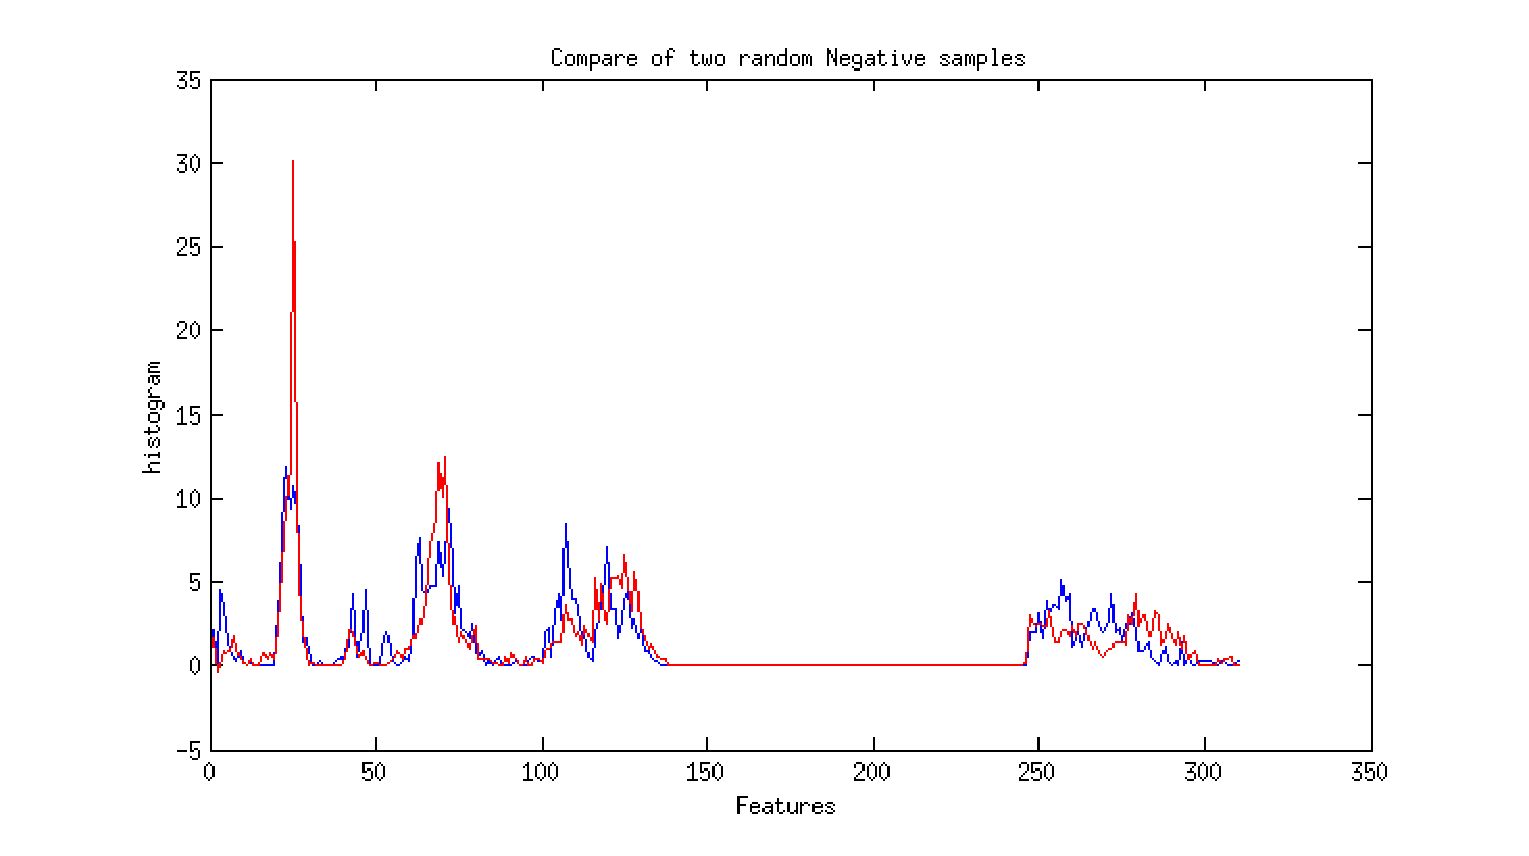
\includegraphics[width=2in,height=2in]{./Figures/CompareNegHis}}
    \subfigure[Compare two random Positive samples.]{\label{ComparePosHist.figure}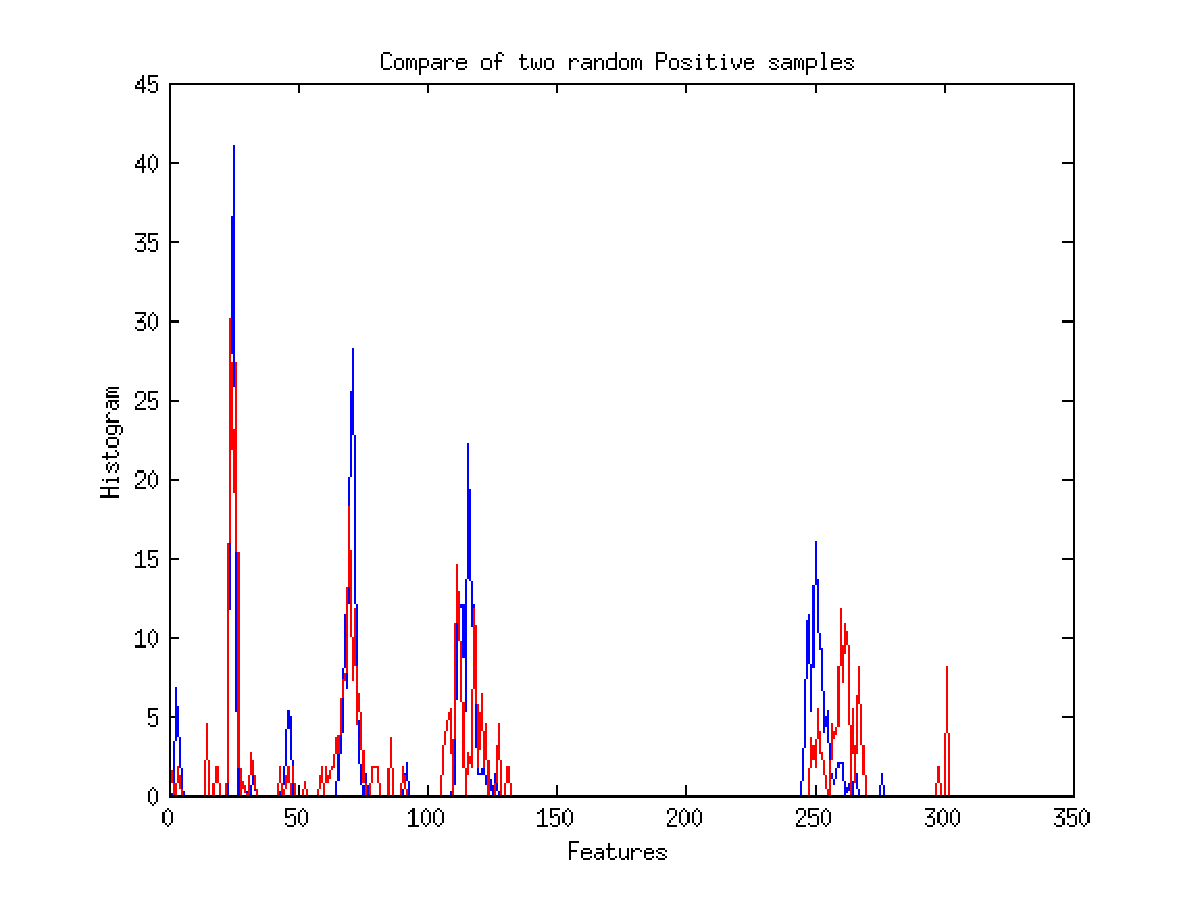
\includegraphics[width=2in,height=2in]{./Figures/ComparePosHist}}
    \subfigure[Distance between random negative samples.]{\label{DistanceOFTwoNegHist.figure}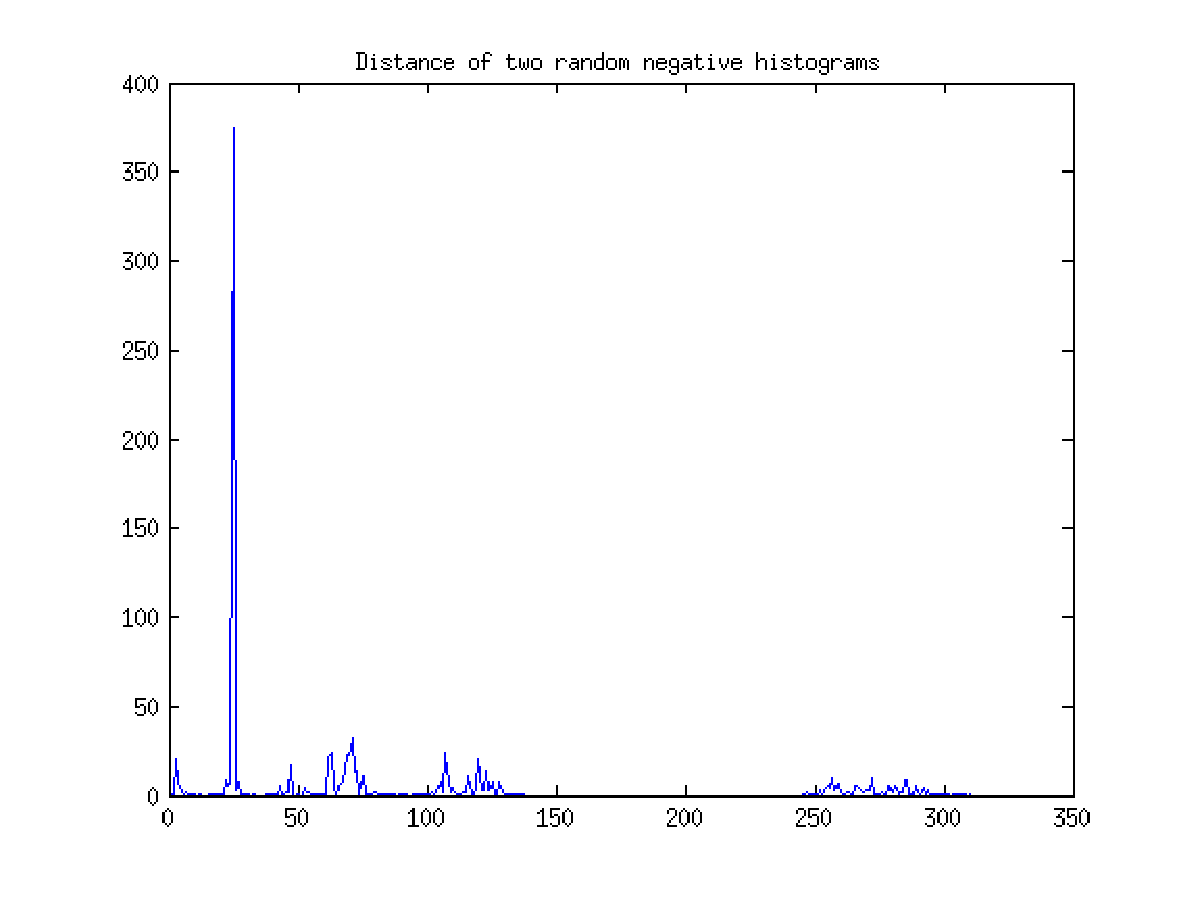
\includegraphics[width=2in,height=2in]{./Figures/DistanceOFTwoNegHist}}
    \subfigure[Distance between random Positive samples.]{\label{DistanceOFTwoPosHist.figure}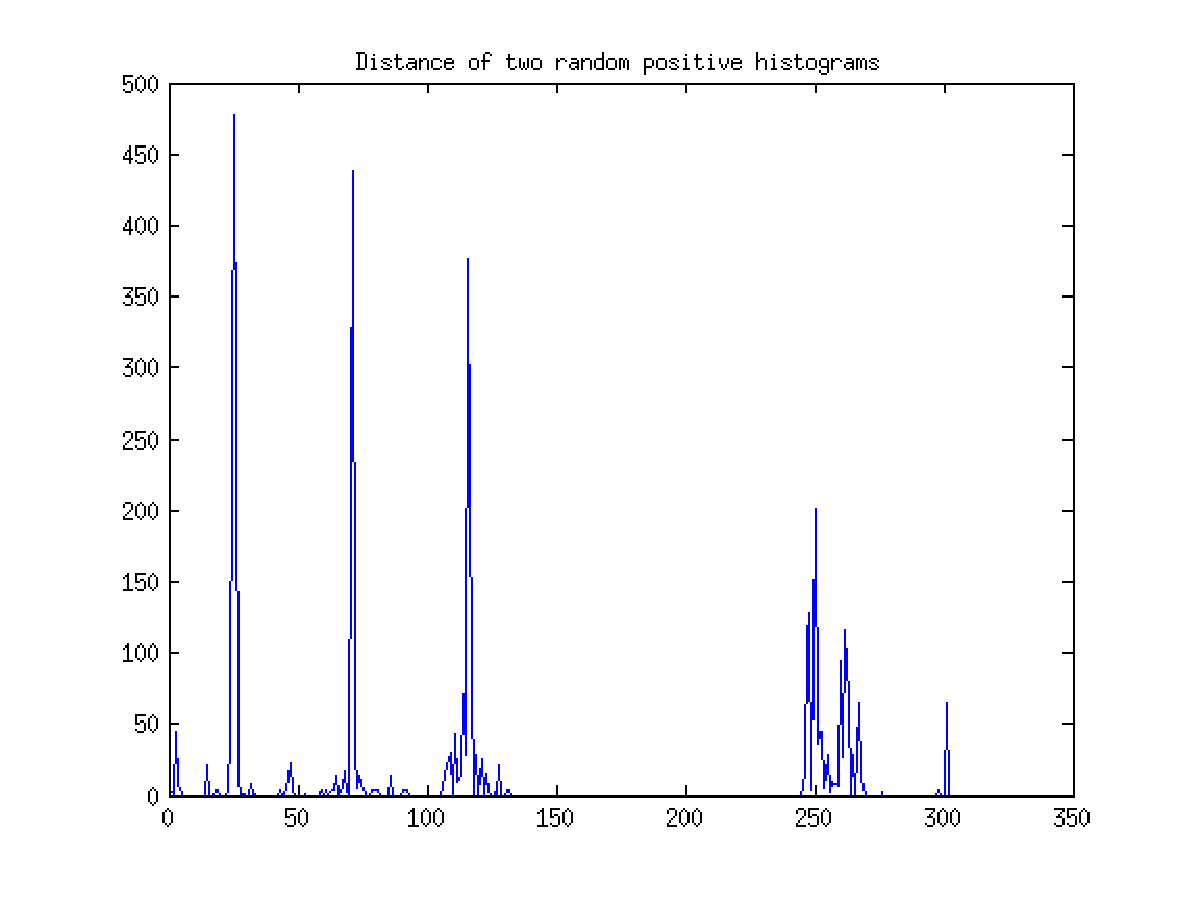
\includegraphics[width=2in,height=2in]{./Figures/DistanceOFTwoPosHist}}
  \end{center}
  \caption[Comparative plots of random samples.]
  {Plots of feature vectors of random positive and negative samples and the euclidean distances between them. This comparison shows the challenge in training a classifier for these samples.}
  \label{ComparativeFVPlot.figure:edge}
\end{figure}
%\begin{figure}
  %\centerpsw{CompareNegHis}{0.65\columnwidth}
  %\caption[Compare two random negative samples]
  %{Two random Negative samples plotted on top of each other to compare.}
  %\label{CompareNegHis.figure} 
%\end{figure}

%\begin{figure}[t]
%\centerpsw{ComparePosHist}{0.65\columnwidth}
%   \caption[Compare two random Positive samples]
%   {Two random Positive samples plotted on top of each other to compare.}
%  \label{ComparePosHist.figure}
%\end{figure}

%\begin{figure}[t]
%  \centerpsw{DistanceOFTwoNegHist}{0.65\columnwidth}
%   \caption[Distance between random negative samples]
%   {Distance between random negative samples.}
%  \label{DistanceOFTwoNegHist.figure}
%\end{figure}

%\begin{figure}[t]
%  \centerpsw{DistanceOFTwoPosHist}{0.65\columnwidth}
%   \caption[Distance between random Positive samples]
%   {Distance between random Positive samples.}
%  \label{DistanceOFTwoPosHist.figure}
%\end{figure}

\begin{figure}[t]
  \centerpsw{DistanceOFPosandNegHist}{0.65\columnwidth}
  \caption[Distance of Positive and Negative samples]
  {Distance between random positive and negative samples.}
  \label{DistanceOFPosandNegHist.figure}
\end{figure}

In order to have a more precise idea about differences between samples, we can also look at the distances between random samples
in the same class and compare them to the distance of samples from different classes. 
Figure ~\ref{DistanceOFTwoNegHist.figure} shows the distance in two random negative samples. 
It should be noticed that the first part of the plot reflects the viewpoint component of the feature vector.
 


And Figure ~\ref{DistanceOFTwoPosHist.figure} is the same plot for positive samples. 
Features extracted for each class can have significant differences as well, which was predictable. 
Considering different surfaces captured as context by these features that can belong to a class causes the differences. 
A positive sample can represent, for instance, the surface of a table or a wall or the meeting region of these 
two surfaces. 
This comparison gives us an idea about how challenging it is to train a classifier for such data.
As mentioned before, it is also vital to put more attention on the positive samples rather than negative ones when training the model. 



Figure ~\ref{DistanceOFPosandNegHist.figure} shows the distance between random positive and negative samples.


\begin{figure}[t]
  \centerpsw{DetailedOverview}{1.1\columnwidth}
  \caption[Detailed Overview of the system]
  {Detailed Overview of the system.}
  \label{DetailedOverview.figure}
\end{figure}

Figure ~\ref{DetailedOverview.figure} shows the whole workflow of the systems with more details comparing to the block diagram in ~\ref{SystemOverview.figure}.
In the next chapter, the setup for the experiment is described, and results are evaluated.


% \section{Experimental Setup}
% \label{ExperimentalSetup.sec}
% Environment setup
% In order to do an evaluation on our method and the model, some experiments are carried out.
% To prepare a dataset for our experiments we needed to capture several pointclouds from different scenes and places which 
% include different object classes.
% 
% 
% To capture pointclouds we used different tools:
% RGBDSLAM \cite{RGBDSLAM} is an open source  package available in ROS. 
% Using this package and kinect sensor with OpenNi driver a 3D model of a scene can be captured. 
% The results are saved as pcd files.
% Pointclouds were captured from different types of places from KTH campus like offices, Kitchens and bathrooms including 
% different types of object that can be found in those places.
% 
% There is also a project in CVAP\footnote{Computer Vision and Active Perception lab.} at KTH called KINECT@HOME \cite{aydemir2012kinect} which is a web based application uses
% kinect out puts to build 3D mesh model of objects and places. 
% A very good property of this system is that people from any part of the world capture their own video with kinect from different 
% places and scenes and post the videos to a server where the 3D reconstruction happens. 
% Through this means a good dataset can be prepared to train and test models.
% Of course, not all of the resulting pointclouds from this database are useful for our purpose due to the content and
% quality, but still there are applicable ones.
% but there were a lot of models that we chose among and 
% converted them to the pointcloud type that was compatible with our system.
% 
% TODO: Silberman's data set.
% 
% Data set
% All resulting pointclouds are saved and based on their content, a name is assigned to them. 
% Then, they are divided into three subsets of train, validation and test. 
% Although, samples from the same pointcloud could be divided into train and validation sets, but we preferred to make them 
% separate even from pointcloud level to be sure of having reliable results. 
% Figure \ref{TrainClouds1.figure:edge} shows full pointclouds with different type of trash bins annotated in them. 
% These are the pointclouds used in experiments.
% Each of these train and validation sets included different category of places.
% Procedure
% 
% 
% \begin{figure} [htp]
%    \begin{center}
%     \subfigure[A partial view of a bathroom.]{\label{TrainClouds1.figure:Bathroom}\includegraphics[width=2in,height=2in]{./Figures/CVAP_Bathroom_6thfloor}}
%     \subfigure[Full pointcloud of a kitchen.]{\label{TrainClouds1.figure:Kitchen4th}\includegraphics[width=2in,height=2in]{./Figures/CVAP_Kitchen_4thFloor}} \\
%     \subfigure[A partial view of a office.]{\label{TrainClouds1.figure:Office607}\includegraphics[width=2in,height=2in]{./Figures/CVAP_Office_607_Desk}}
%     \subfigure[A full pointcloud of an office.]{\label{TrainClouds1.figure:Office518}\includegraphics[width=2in,height=2in]{./Figures/CVAP_Office_518}} \\
%     \subfigure[A full pointcloud of another kitchen in the same building.]{\label{TrainClouds1.figure:Kitchen6th}\includegraphics[width=2in,height=2in]{./Figures/CVAP_Kitchen_6thFloor}}
%     \subfigure[A partial view of an office with lots of missing points.]{\label{TrainClouds1.figure:TestCloud}\includegraphics[width=2in,height=2in]{./Figures/TeastCloudAnootaion}} \\
%   \end{center}
%   \caption[Train set pointclouds]
%   {Point cloud used for extracting train samples with trash bin annotations. Bins are in different types and locations.(best viewed in color)}
%   \label{TrainClouds1.figure:edge}
% \end{figure}
% 
% Table \ref{Objects.table} includes names of four different object classes used in experiments and the number of train samples extracted for each of them.
% It also shows what fraction of those samples were positive samples that are actually samples captured from context point blobs.
% 
% 
% \begin{table}
% \centering
% \caption
% [Object classes used in experiments.]
% {Object classes used in experiments with number of samples extracted for each of them for training and ratio of positive samples in them.}
% \label{Objects.table}
% \begin{tabular}{|c|c|c|c|c|}
% \hline
% \multicolumn{2}{|c|}{Object} & \#Train samples & \#Positive Train samples & Ratio \\
% \hline
%       1 & Trash Bin & 142150 & 2493 & 1.7 \\
% \hline
%       2 & Telephone   & 119725 & 554  & 0.4 \\
% \hline
%       3 & Mouse     & 286825 & 1541 & 0.5 \\
% \hline
%       4 & Wiper     & 170025 & 3086 & 1.8 \\
% \hline
% 
% \end{tabular}
% \end{table}
% 
% 
% In experiments with four different object categories mentioned in table \ref{Objects.table} few different scenes are considered to capture train pointclouds from.
% For each scene, a number of different location settings for objects are captured in different point cloud (figures \ref{TrainClouds2.figure:tmt1} and \ref{TrainClouds2.figure:tmt2}).
% Therefore, in the resulting train set each object has a number of instances in different scenes.
% 
% \begin{figure} [htp]
%    \begin{center}
%     \subfigure[Partial cloud including telephone, mouse and trash bin.]{\label{TrainClouds2.figure:tmt1}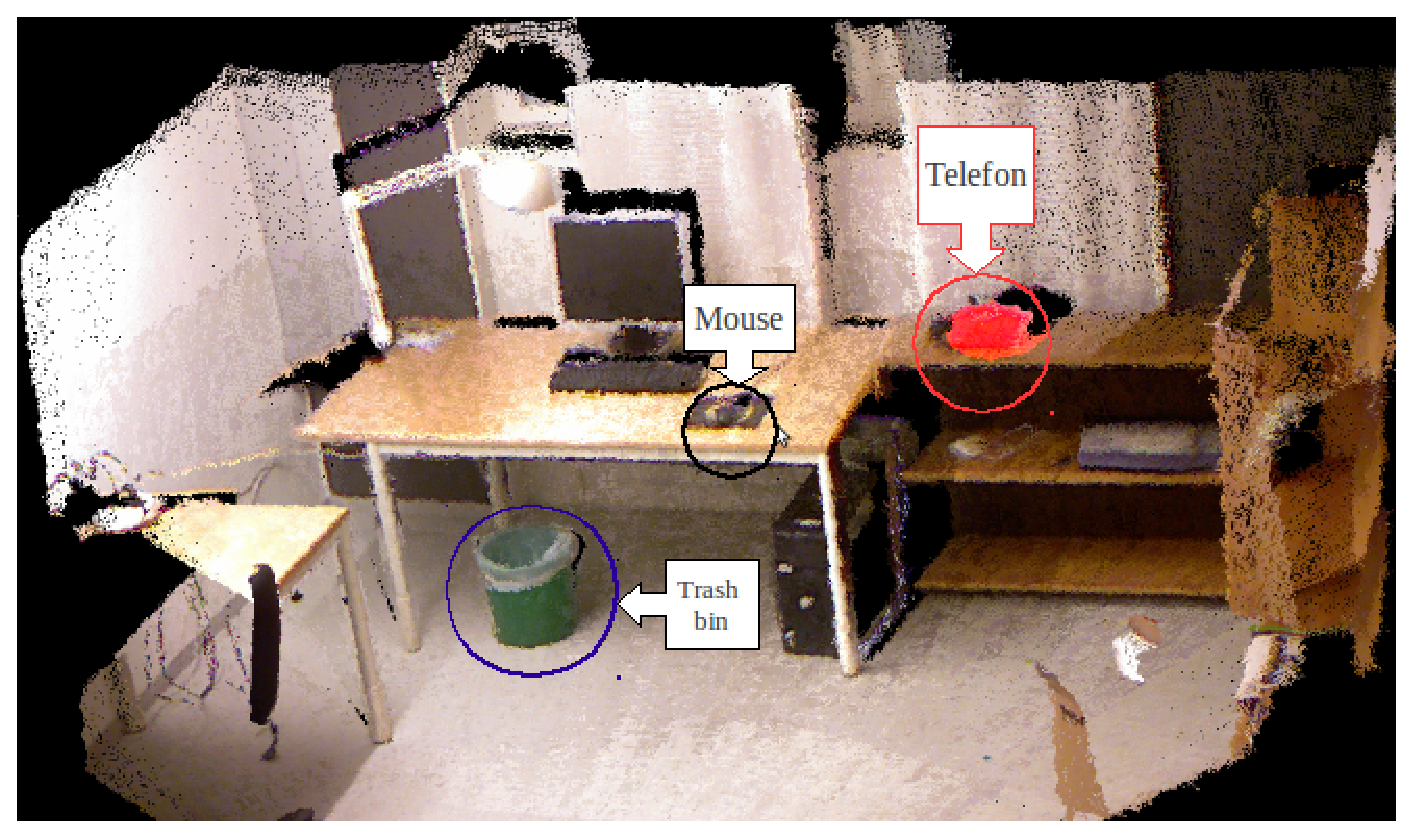
\includegraphics[width=2in,height=2in]{./Figures/518_1_telefon_labels}}
%     \subfigure[The same scene with different location of the objects.]{\label{TrainClouds2.figure:tmt2}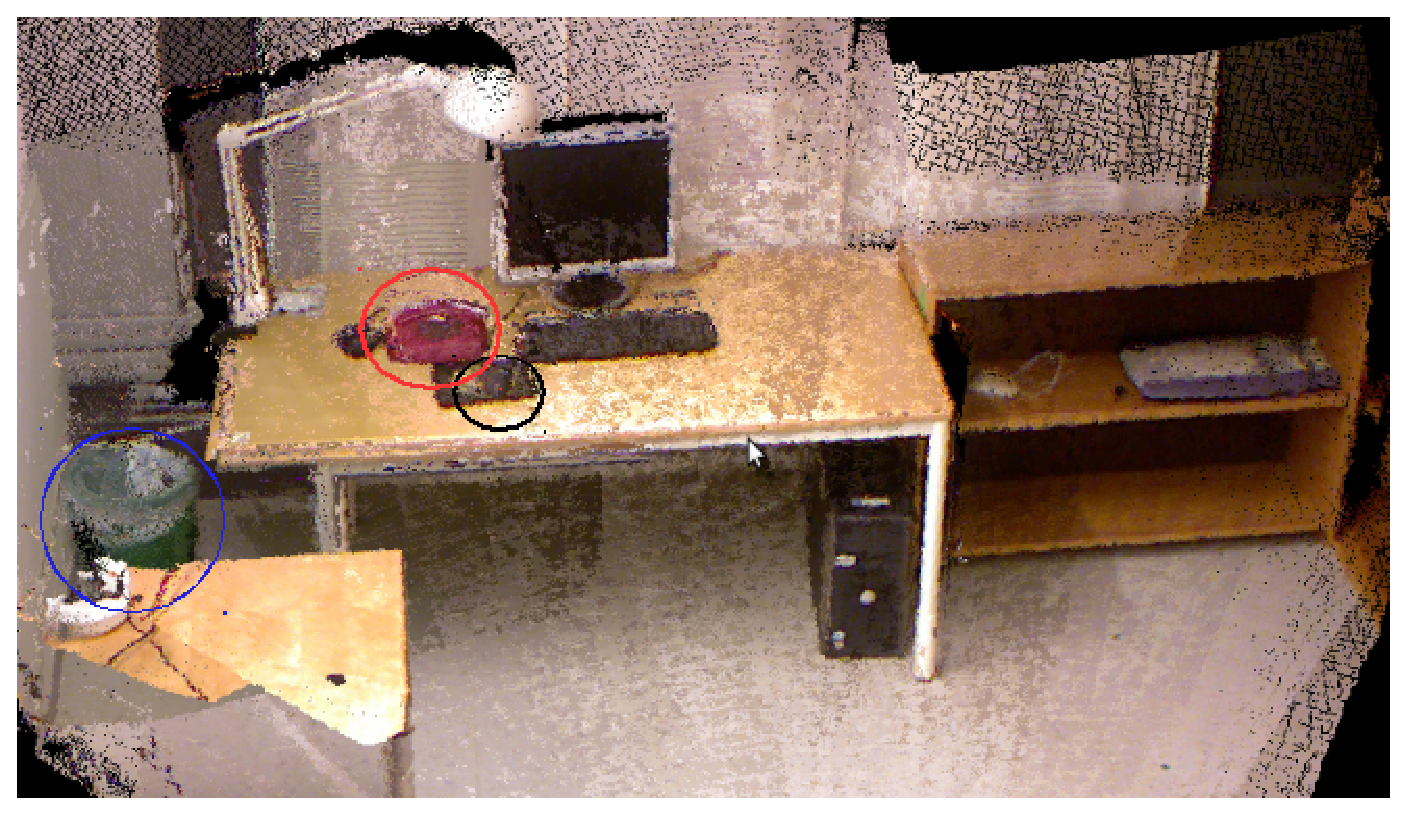
\includegraphics[width=2in,height=2in]{./Figures/518_3_labels}} \\
%     \subfigure[Partial cloud including white board wipers.]{\label{TrainClouds2.figure:wiper}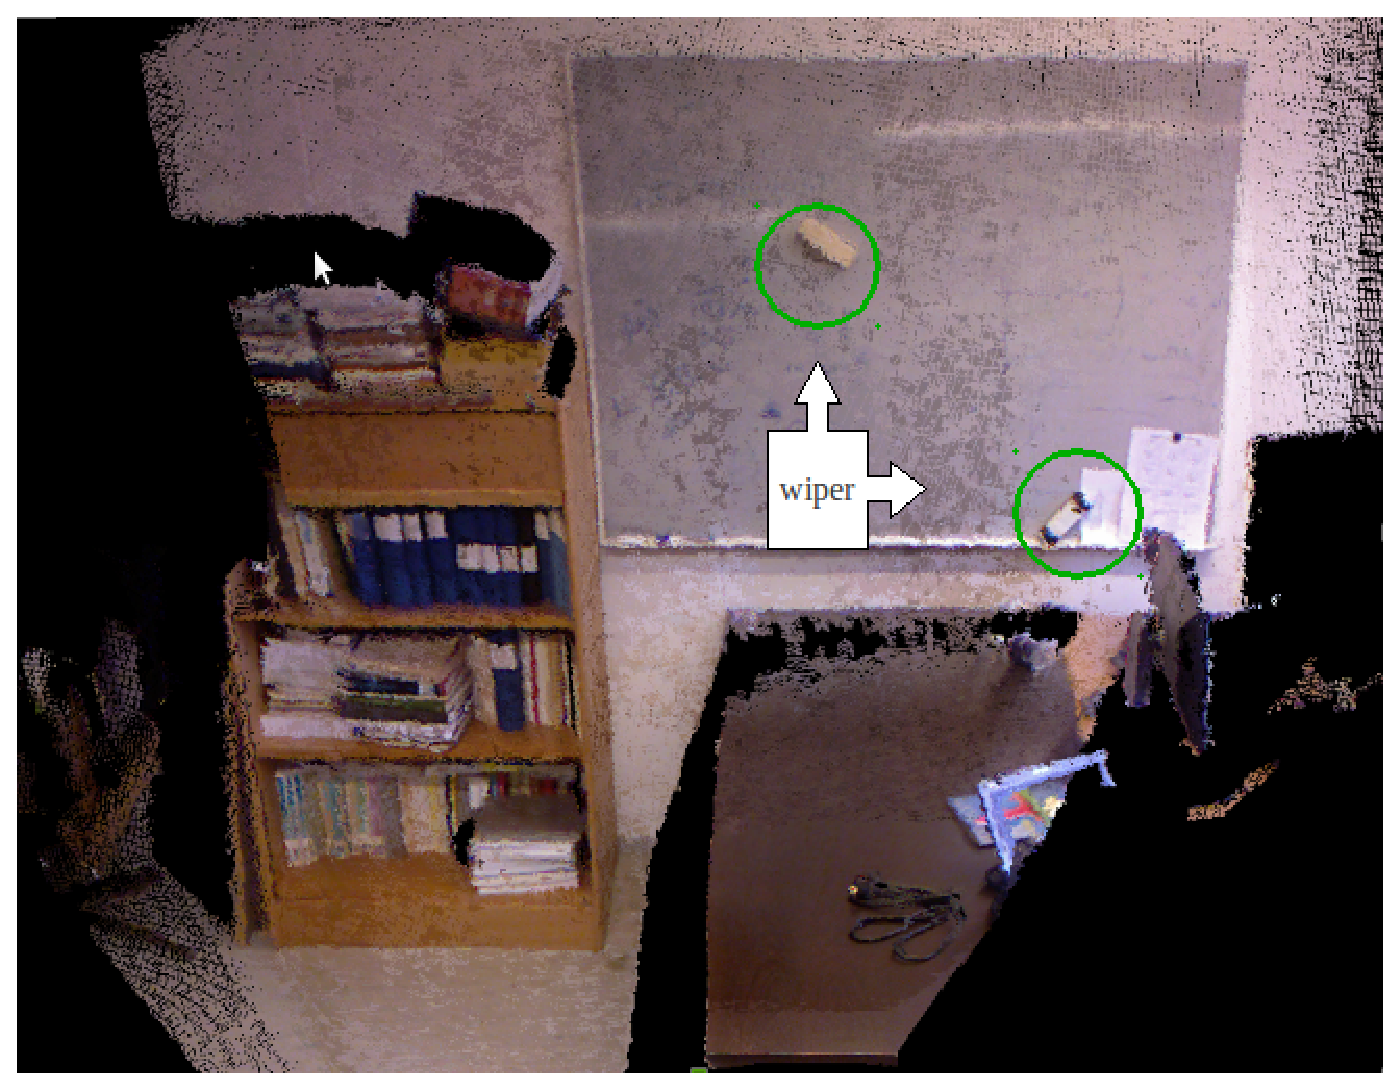
\includegraphics[width=2in,height=2in]{./Figures/wiper_labels}}
%     \subfigure[A partial cloud including several instances of 3 object categories.]{\label{TrainClouds2.figure:tmt3}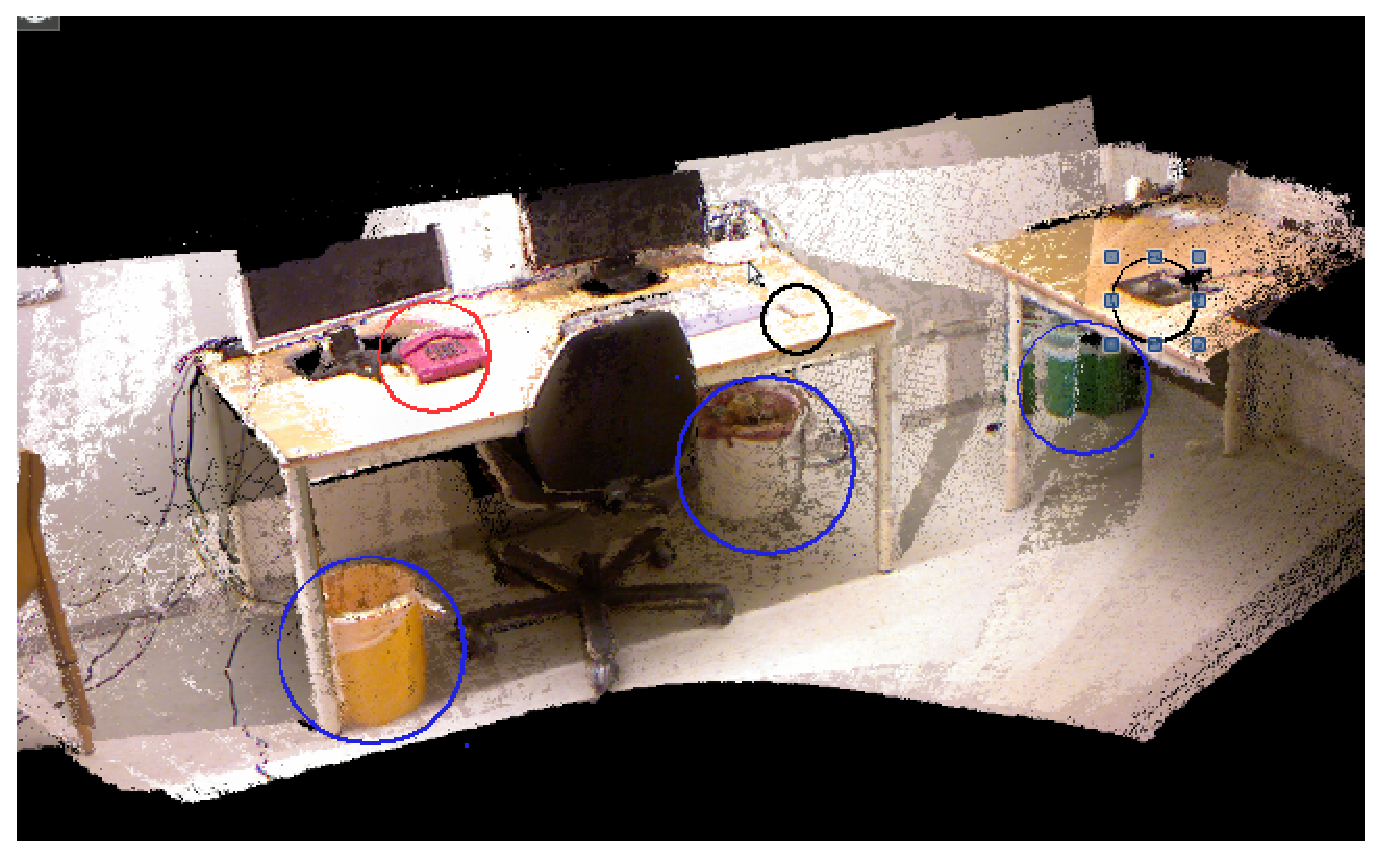
\includegraphics[width=2in,height=2in]{./Figures/518_4_labels}} \\
%   \end{center}
%   \caption[Train set pointclouds including four different object class.]
%   {Partial pointclouds including four object categories: trash bin(marked with blue circles), mouse(back circles), telephone(red circles) and wiper(green circles) in different location settings used in training.(best viewed in color)}
%   \label{TrainClouds2.figure:edge}
% \end{figure}
% 
% 
% 
% 
% After acquiring the pointclouds, some scripts were used that picks the pointcloud from the input dataset 
% and load them into PreProcess module and saves the results of each pointcloud separately in a useful way into the automatically
% generated environment. 
% Then the annotation tool were used to annotate objects of interest in the pointclouds. 
% All pointclouds were annotated with present objects of interest, regardless of them being in the train set or validation to 
% make evaluation possible on ones used for test as well. 
% Although in validation we would not be using labels from annotation until the end of classification, 
% this information is needed for evaluation which would be described later in next Section ~\ref{Results.sec}.
% 
% 
% In the next step, another script picks annotated clouds and their normals (estimated in PreProcess) into Feature extract 
% and  resulting feature vectors are saved in a folder for the corresponding object class under train or validation set, regarding
% which set their source pointcloud belong to.
% Then, a subset is randomly selected from the train samples in a way that includes all the positive samples and sevral times more of 
%  negative samples to make the train set.
% In first experiments for Trash bin we have used train sets with 10 percent positive and 90 percent negative samples.
% In later experiments and for other objects train sets are generated with all extracted positive samples and two times more of negative samples.
% In these experiments positive sample have a 33\% share in the train set.
% 
% At this point, all data sets are scaled with the same parameters, then the scaled train set is given to SVM train 
% to make the models for each of the object class's context. 
% During training, different values for the parameters are considered, and each resulting model is applied on samples from validation
% set. 
% Classification results with different examined values of these parameters are compared and best models are selected. 
% The results and evaluation procedure are discussed in Section ~\ref{Results.sec}.
% 
% \section{Results}
% \label{Results.sec}
% Definitions and metrics
% In this section, we take a look at some results and analyze and evaluate them to see how good our method performs.
% 
% \subsection{Evaluation metric}
% \label{EvaluationMetric.ssec}
% 
% As mentioned before there could be negative samples in train set that are labeled as negative just because they were not captured 
% from a neighborhood of an annotated object while they have very similar features to positive samples. 
% Such samples need to be predicted as positive. 
% 
% Here we define the metric and evaluation method that we considered in this work.
% Metrics such as accuracy or prediction is not something that can show the performance of our system.
% Accuracy is measuring number of samples that are correctly classified with respect to the total number of samples.
% Here we do not have direct access to the number of correct classification. 
% 
% Based on the problem definition, we are looking for possible context of an object, which regards to the locations that an 
% object is expected to be found, not just location that an object is present in.
% Intuitively, set of points that belong to an actual object (if there is an actual object in the scene) is a subset of all 
% possible object points in that scene.
% Therefore, actual object points ($Lp$) are a subset of predicted positive points ($Pp$) if the model and classifier perform 
% well (equation \ref{Lp-PpRelation.eq}).
% 
% \begin{equation}
%  \label{Lp-PpRelation.eq}
%  Lp \subset Pp
% \end{equation}
% 
% In other words, from a good result, we expect any random point sampling which is an actual object point to be within 
% predicted positive points.
% Similar metric is used in recently published and praised work \cite{aydemir2012_3Dcontext}.
% if the predictions give us points of the pointcloud where there is a high probability of finding the object, it
% would be what we want. 
% The point here is, that the location of the object would be a subset of this predicted set. 
% With this definition there would be a problem: if all points get predicted as positive then actual object points would 
% definitely be a subset of it, while our classification has failed.
% As a result, we define a good result as predicted set of locations that reduces our search space for the object as much as 
% possible while it preserves the high probability of finding the object.
% 
% Equation ~\ref{Eval.eq} shows the evaluation metric, where $E(\tau)$ is the the value of the metric with respect to a 
% probability threshold $\tau$. 
% This threshold sets the boundary for the lowest probability value that the prediction for a point should have to be 
% considered as positive. 
% This threshold is assigned with a value in a loop that as a result in each iteration a top fraction of the samples are being 
% picked and analyzed. 
% The threshold is computed based on an increasing number of considered points.
% For instance, the threshold takes a value that separates the top five percent of the points with respect to their prediction 
% value.
% Then, the probability of having the object in this fraction of points is computed.
% 
% 
% $Pp_{\tau}$ is predicted positive sample with respect to the value of the threshold and $n(x)$ is the number of 
% members in the set $x$, e.g. $n(Lp)$ it is number of points belonging to $Lp$. $Lp$ is the 
% labeled positive points in the data-set or in other word the annotated object.
% 
% \begin{equation}
%  \label{Eval.eq}
%     E(\tau) = \frac{n({Pp_{\tau}} \cap {Lp})}{n(Lp)} 
% \end{equation}
% 
% This value is between zero and one, and a value closer to one, while the threshold is high enough, shows a better result.
% This metric is also used in experiments to find the best models and parameters. 
% Here we also translate the sample base results into point base which means the result is assigned to the point for which 
% the sample is taken.
% Therefore, the prediction directly shows if a candidate OPoint is a possible object point or not.
% 
% Figure ~\ref{Eval80ExperimentTop10.figure} shows the value of $E$ for top ten percent of the points with respect to their 
% prediction probability in experiments with 80 different configuration of weights and gamma.
% As it can be seen the results look pretty good.
% 
% \begin{figure}[t]
%   \centerpsw{Eval80ExperimentTop10}{0.65\columnwidth}
%   \caption[Evaluation result of 80 experiments]
%   {Top 10 percent of positive predictions in experiments with 80 different configurations for parameters.}
%   \label{Eval80ExperimentTop10.figure}
% \end{figure}
% 
% \subsection{Evaluation results}
% \label{EvaluationResult.ssec}
% 
% \begin{figure}[t]
%   \centerpsw{evalMorevalues}{0.85\columnwidth}
%   \caption[Evaluation diagram for experiments with Gaussian kernel.]
%   {Evaluation diagram for experiments with Gaussian kernel. Each line corresponds to a value for w-1.(Best viewed in color.)}
%   \label{evalSevenExp.figure}
% \end{figure}
% We have two sets of experiments, in the first one the learning is done using one Gaussian kernel on the whole feature vector.
% In the second set we used double kernel of type chi-square with equal weights.
% One is applied on first two field of the feature vector(orientation and height) and the other on the VFH part.
% 
% Figure ~\ref{evalSevenExp.figure} shows this evaluation for seven experiments with different values for w(-1) which is the 
% parameter setting the weight of the negative class in SVM classifier.
% In these experiments a single Gaussian kernel is employed to build the model of trash bin context.
% The value is depicted with respect to the fraction of points considered.
% 
% Considering best models, it can be inferred from the curves that for instance, considering top five percent of the points 
% contains twenty percent of the object which is a good result. 
% In other words, reducing the the search space to only 5 percent we still have four time chance of finding the object.
% 
% 
% 
% Figure ~\ref{TrashPrediction.figure:edge} shows the prediction of trash bin context on a full pointcloud of an office. 
% The marked region shows the points with highest probability values(top 1\%).
% This predicted context reaches the trash bin which is present in the scene when the probability threshold reaches the 
% probability of top 5\% of points.
% The interesting point is that this trained model is suggesting that corner is the best location in this scene to find a 
% trash bin or put one (based on the train data).
% 
% \begin{figure} [htp]
%    \begin{center}
%     \subfigure[A test pointcloud for trash bin model, marked region with red circle is the predicted context.]{\label{TrashPrediction.figure:full}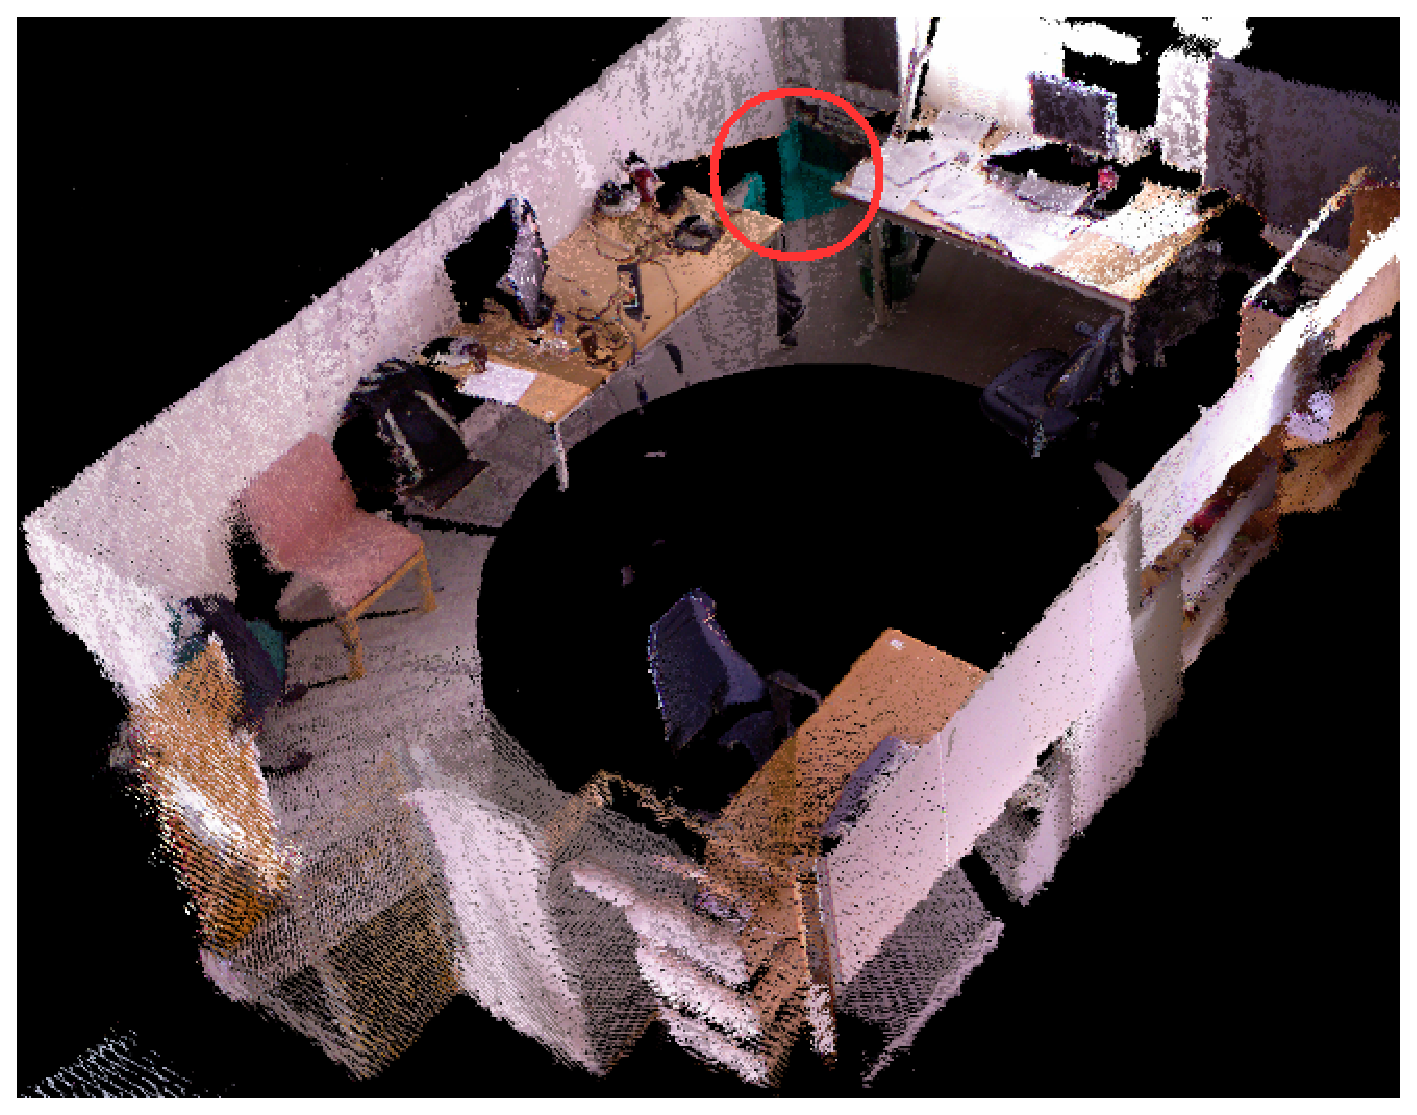
\includegraphics[width=3in,height=3in]{./Figures/TrashBinPrediction}}
%     \subfigure[Focused to predicted region.]{\label{TrashPrediction.figure:focused}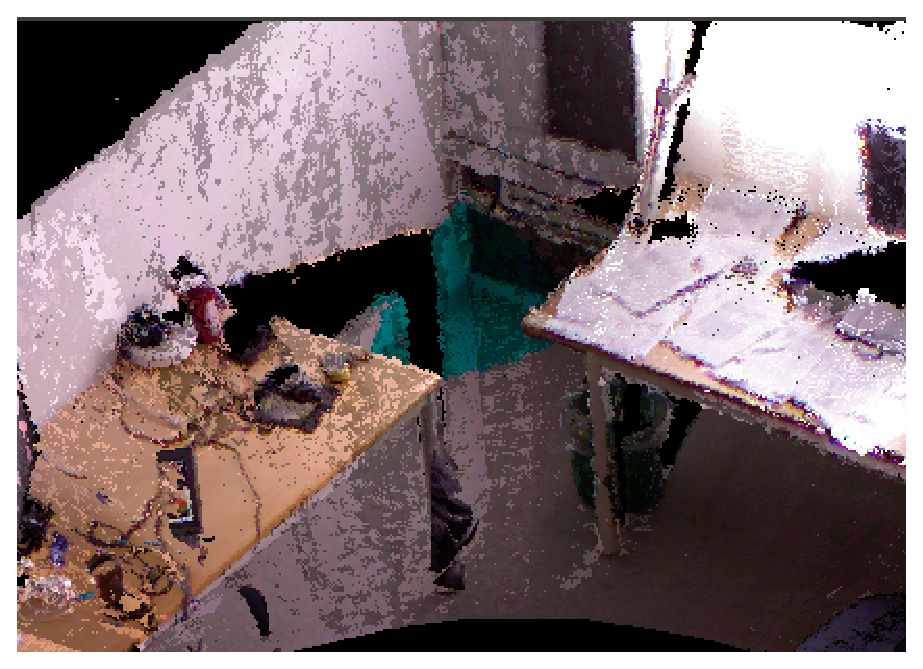
\includegraphics[width=3in,height=3in]{./Figures/TrashBinPrediction_focused}} \\
%   \end{center}
%   \caption[Prediction of Trash bin model.]
%   {Prediction of Trash bin context on a full pointcloud of an office. The marked region shows the points with highest probability values(top 1\%).(best viewed in color)}
%   \label{TrashPrediction.figure:edge}
% \end{figure}
% 
% In later experiments that we used multi kernel of type chi-square, there was a significant improvement on the results.
% As the first two fields of our feature vector are two float values and the rest is histogram, they are to be treaded 
% in different ways.
% So we separated the kernels applied on each of these parts.
% The visualized results of predictions using these kernels with equal weights are shown in Figure ~\ref{ContextPrediction_518_1.figure:edge} 
% for the four object we used in these experiments.
% 
% \begin{figure} [htp]
%    \begin{center}
%     \subfigure[Predicted context for Mouse.]{\label{ContextPrediction_518_1.figure:wiper}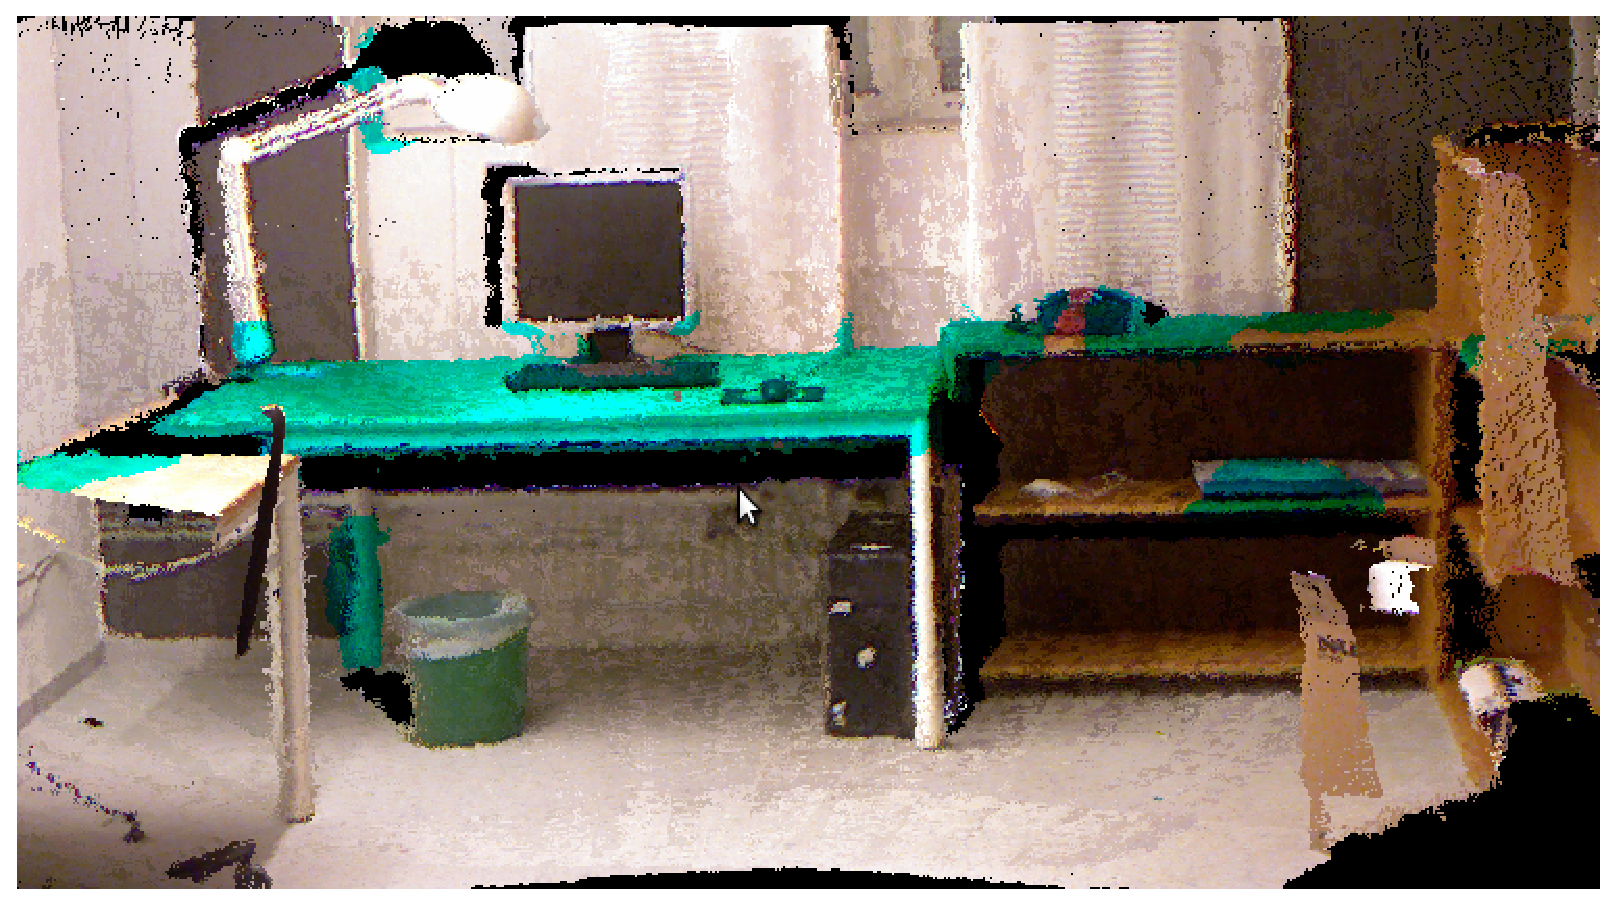
\includegraphics[width=2in,height=2in]{./Figures/518_1_MousePrediction_c1g0}}
%     \subfigure[Predicted context for white-board wiper.]{\label{ContextPrediction_518_1.figure:mouse}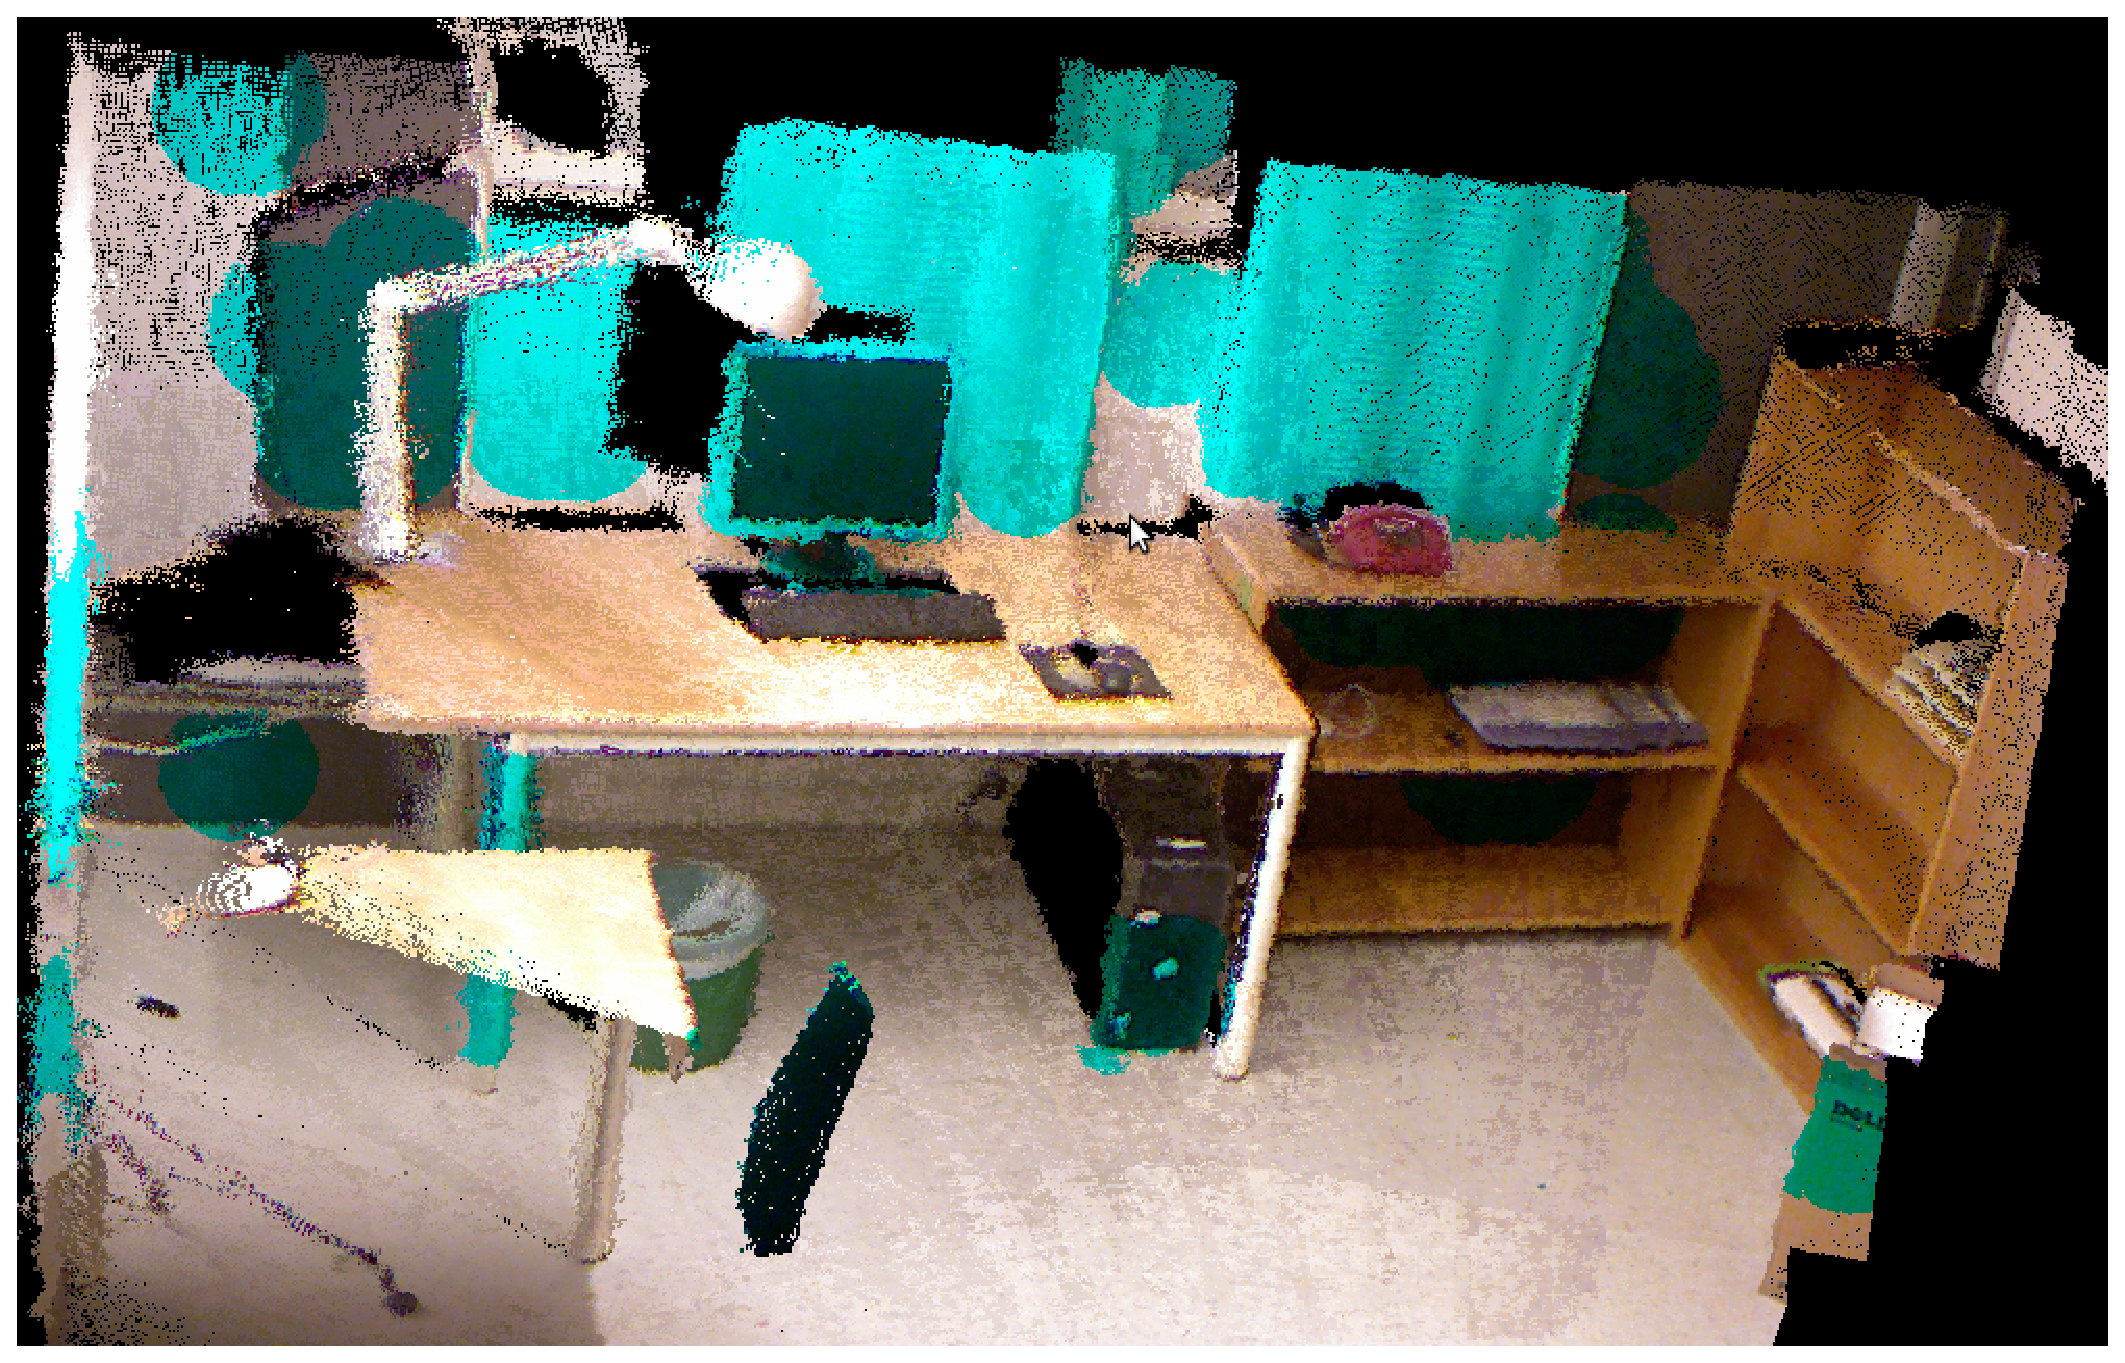
\includegraphics[width=2in,height=2in]{./Figures/518_1_WiperPrediction_c1g0}} \\
%     \subfigure[Predicted context for Telephone.]{\label{ContextPrediction_518_1.figure:Telephone}\includegraphics[width=2in,height=2in]{./Figures/518_1_TelefonPrediction_c1g0}}
%     \subfigure[Predicted context for Trash Bin.]{\label{ContextPrediction_518_1.figure:TrashBin}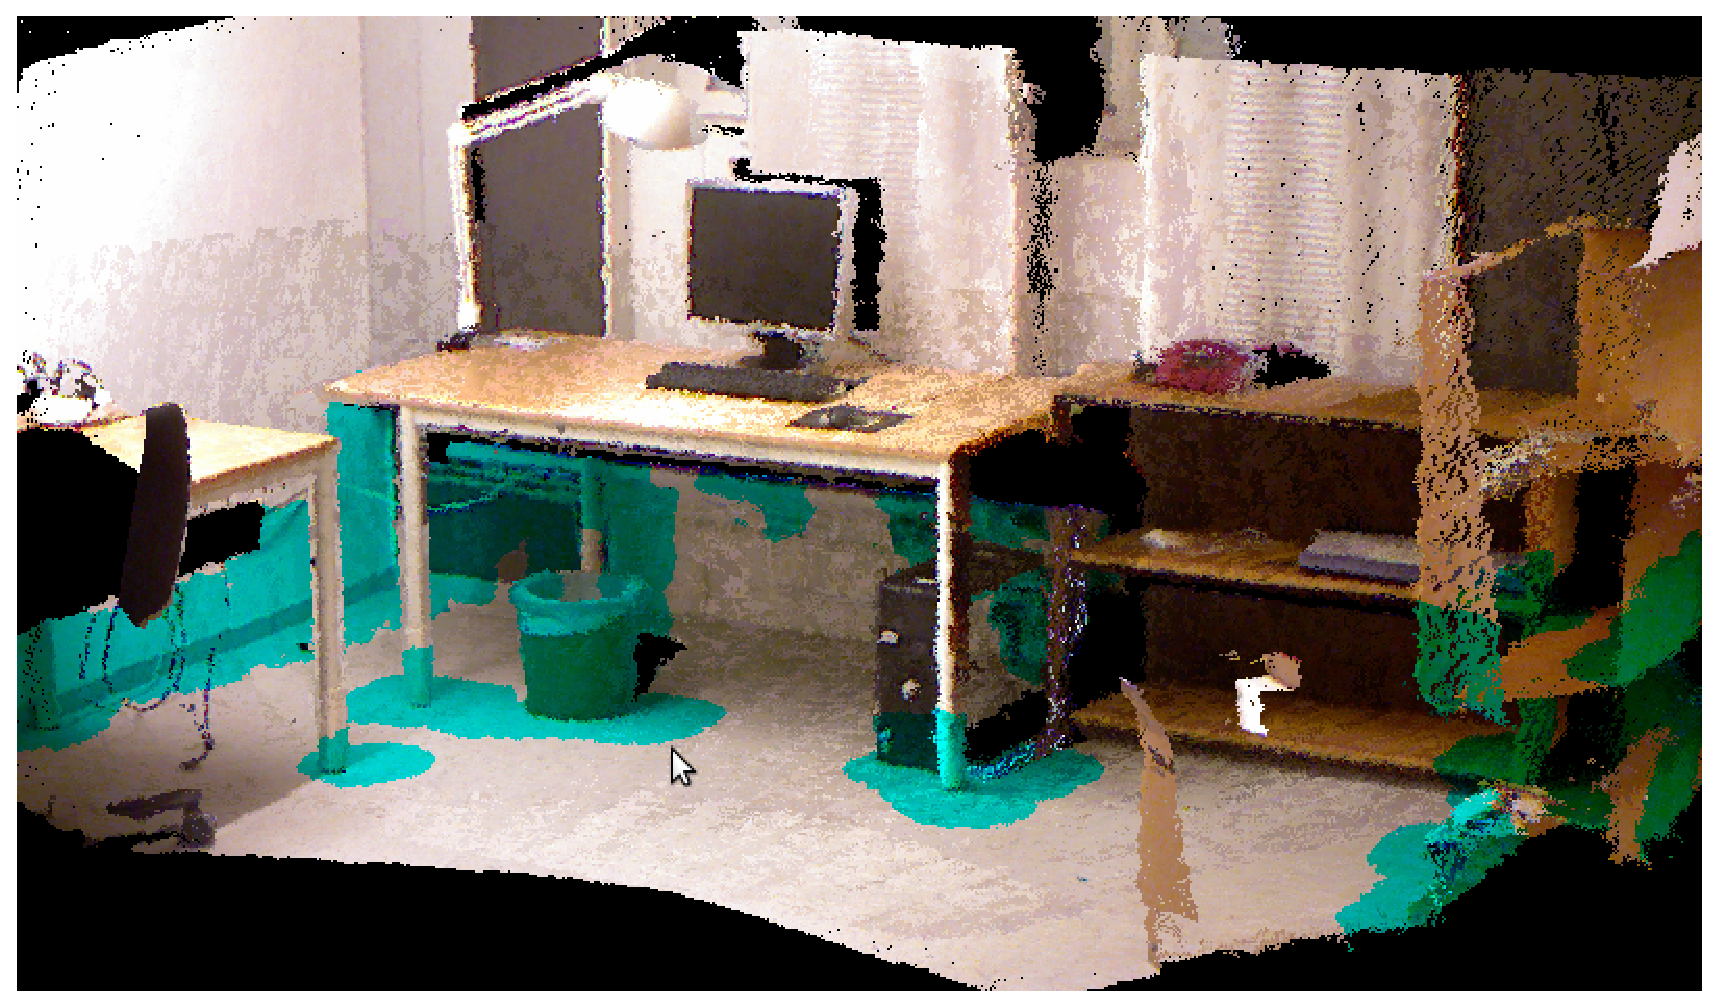
\includegraphics[width=2in,height=2in]{./Figures/518_1_TrashBinPrediction_c1g0}} \\
%   \end{center}
%   \caption[Visualization of context model prediction on sample cloud 1 from validation set.]
%   {Visualization of context model prediction on sample cloud 1 as a validation cloud, for four objects. The key point predicted as positive and the blob around it is projected on the pointcloud in cyan color.(best viewed in color)}
%   \label{ContextPrediction_518_1.figure:edge}
% \end{figure}
% 
% In Figure ~\ref{ContextPrediction_518_1.figure:edge}, the predicted contexts of four object used in experiments 
% are projected on the pointcloud of an office.
% It should be noticed that the regions shown in cyan, are blobs with a key point in the center which is predicted as 
% context.
% 
% The corresponding evaluation values for results shown in Figure ~\ref{ContextPrediction_518_1.figure:edge} are depicted
% in Figure ~\ref{Eval_518_1.figure}.
% A simple comparison between curves in this figure and Figure ~\ref{evalSevenExp.figure} shows the improvement of the 
% results.
% 
% \begin{figure}
%   \begin{center}
%    \centerpsw{Eval4Objects}{0.85\columnwidth}
%   \caption[Evaluation results for four object classes.]
%   {Evaluation results of context prediction for four objects Mouse, Telephone, Trash Bin and wiper. These results are from experiments using chi-square multi kernel.}
%   \label{Eval_518_1.figure}
%   \end{center}
% \end{figure}
% 
% To compare the performance of the system regarding each of these four object class, the values of $E$ in a certain 
% ratio of selected points with respect to all points in the pointcloud is considered for each of these object classes.
% Table ~\ref{performance.table} contains these values for the ratio of top 5\%.
% 
% \begin{table}
% \centering
% \caption
% [Performance of the system for four object classes.]
% {Performance of the system for four object classes.}
% \label{performance.table}
% \begin{tabular}{|c|c|c|}
% \hline
% Object & E in top 5\% of points & The ratio that E reaches to 1 \\
% \hline
%       Mouse & 0.6667 & 15 \\
% \hline
%       Telephone & 1 & 5 \\
% \hline
%       Trash Bin & 0.3333 &  40\\
% \hline
%       Wiper & 0.42 & 60 \\
% \hline
% \end{tabular}
% \end{table}
% 
% As it can be seen in table ~\ref{performance.table}, the best performance of the system is for Telephone and after 
% that for Mouse.
% These two are often found in a similar context which can be a good reason for these results.
% The context for trash bin, at least based on our train set, can have wider variety compared to mouse and telephone.
% That is why its performance value is the lowest.
% 
% But for wiper, as the context is usually similar it can not be a good explanation.
% In the wiper case, the reason for its low performance should be the wide range of heights this object can be located in.
% We consider the height as an important feature in building our models which makes it very effective.
% The effectiveness of height seems to be not so useful in the case of wiper.
% A solution can be using smaller weights for the height feature in modeling these object classes.
% 
% \begin{figure} [htp]
%    \begin{center}
%     \subfigure[Predicted context for Mouse.]{\label{ContextPrediction_Test_512.figure:wiper}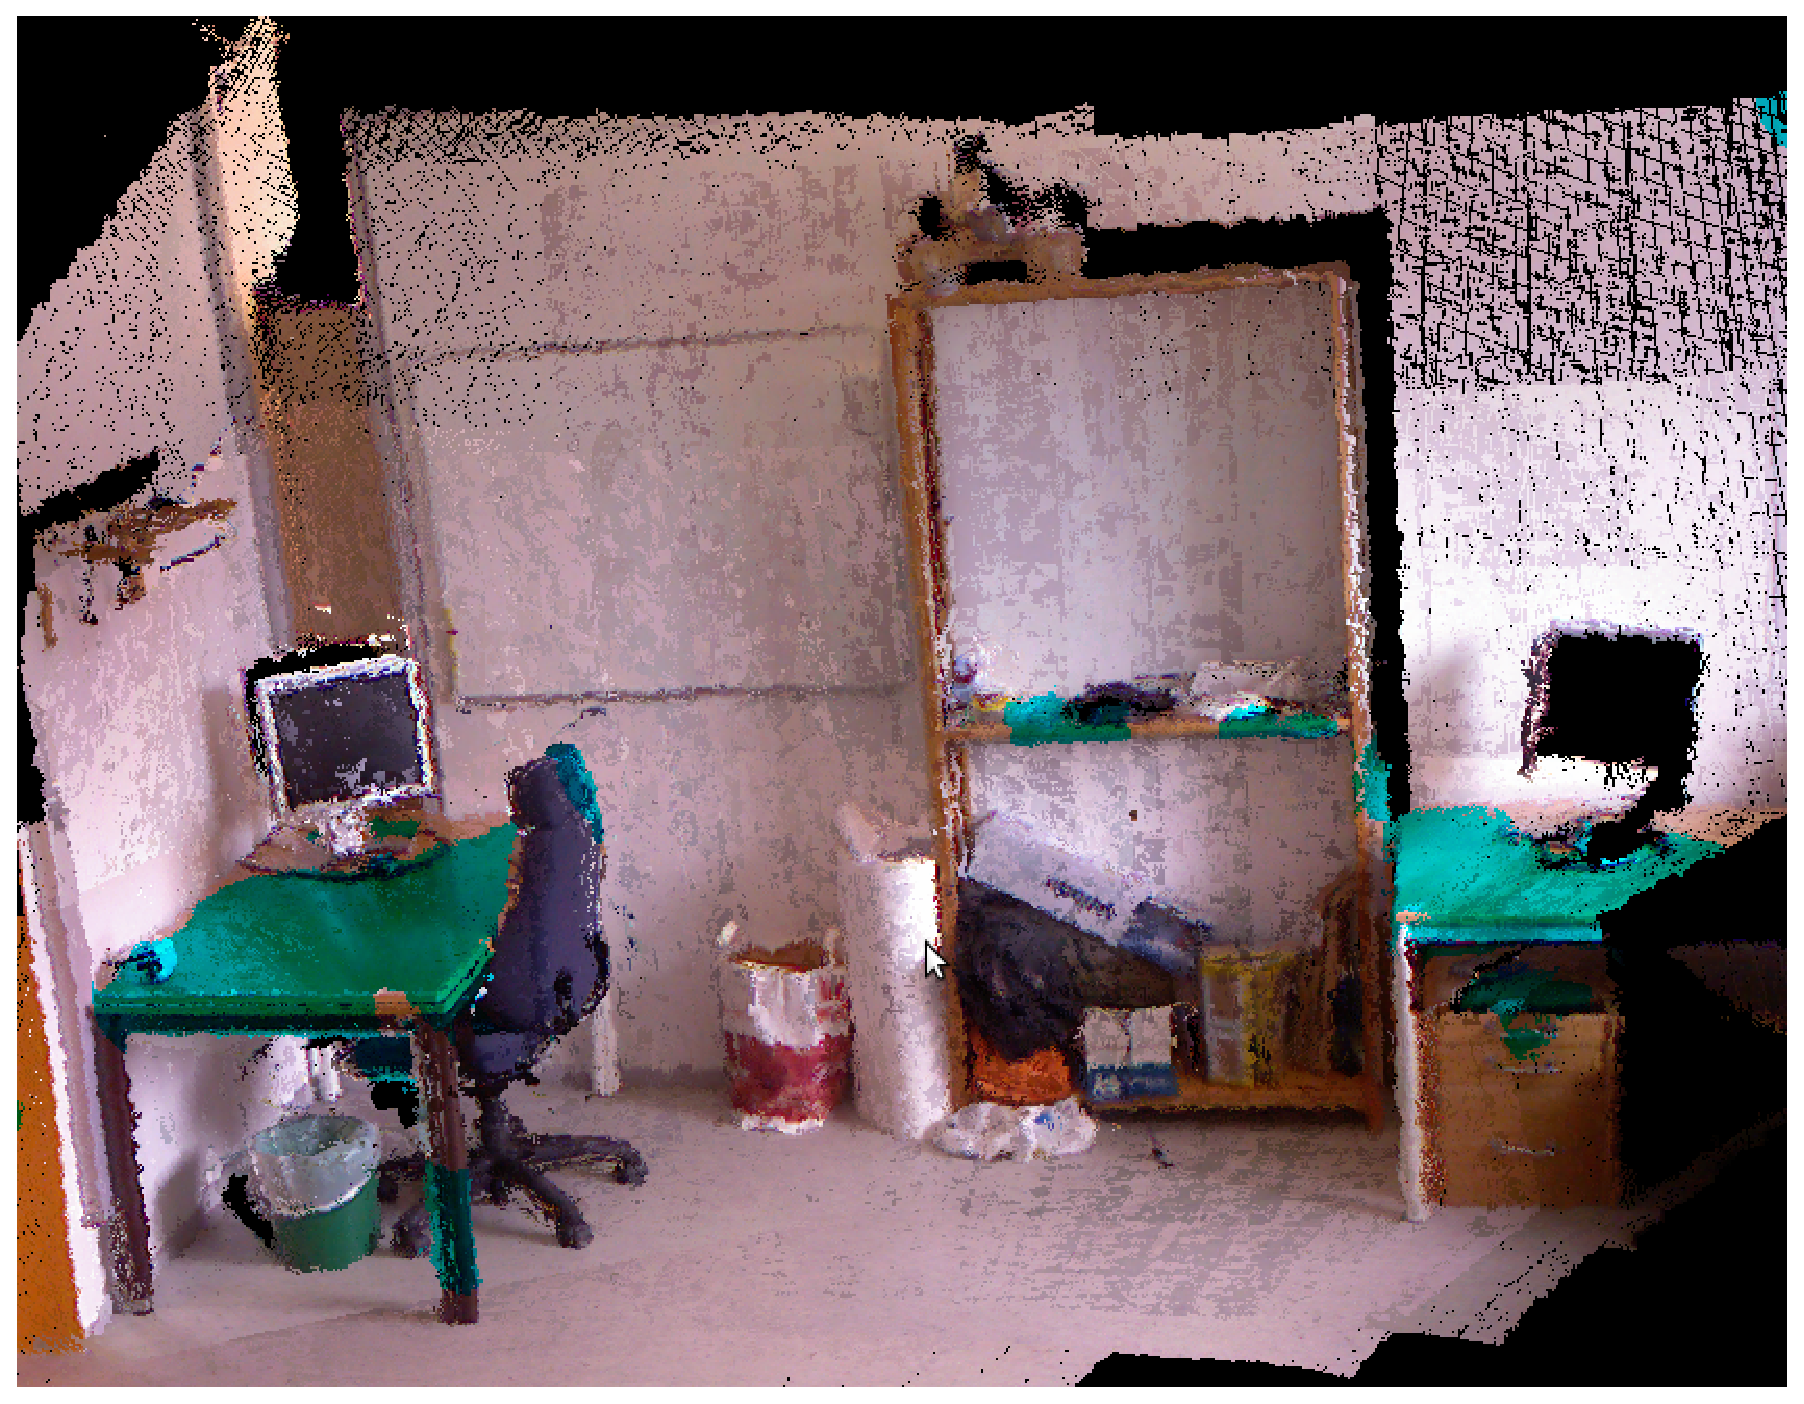
\includegraphics[width=2in,height=2in]{./Figures/Test21_2_13MousePredict_c1g0.eps}}
%     \subfigure[Predicted context for white-board wiper.]{\label{ContextPrediction_Test_512.figure:mouse}\includegraphics[width=2in,height=2in]{./Figures/Test_wiperPrediction.eps}} \\
%     \subfigure[Predicted context for Telephone.]{\label{ContextPrediction_Test_512.figure:Telephone}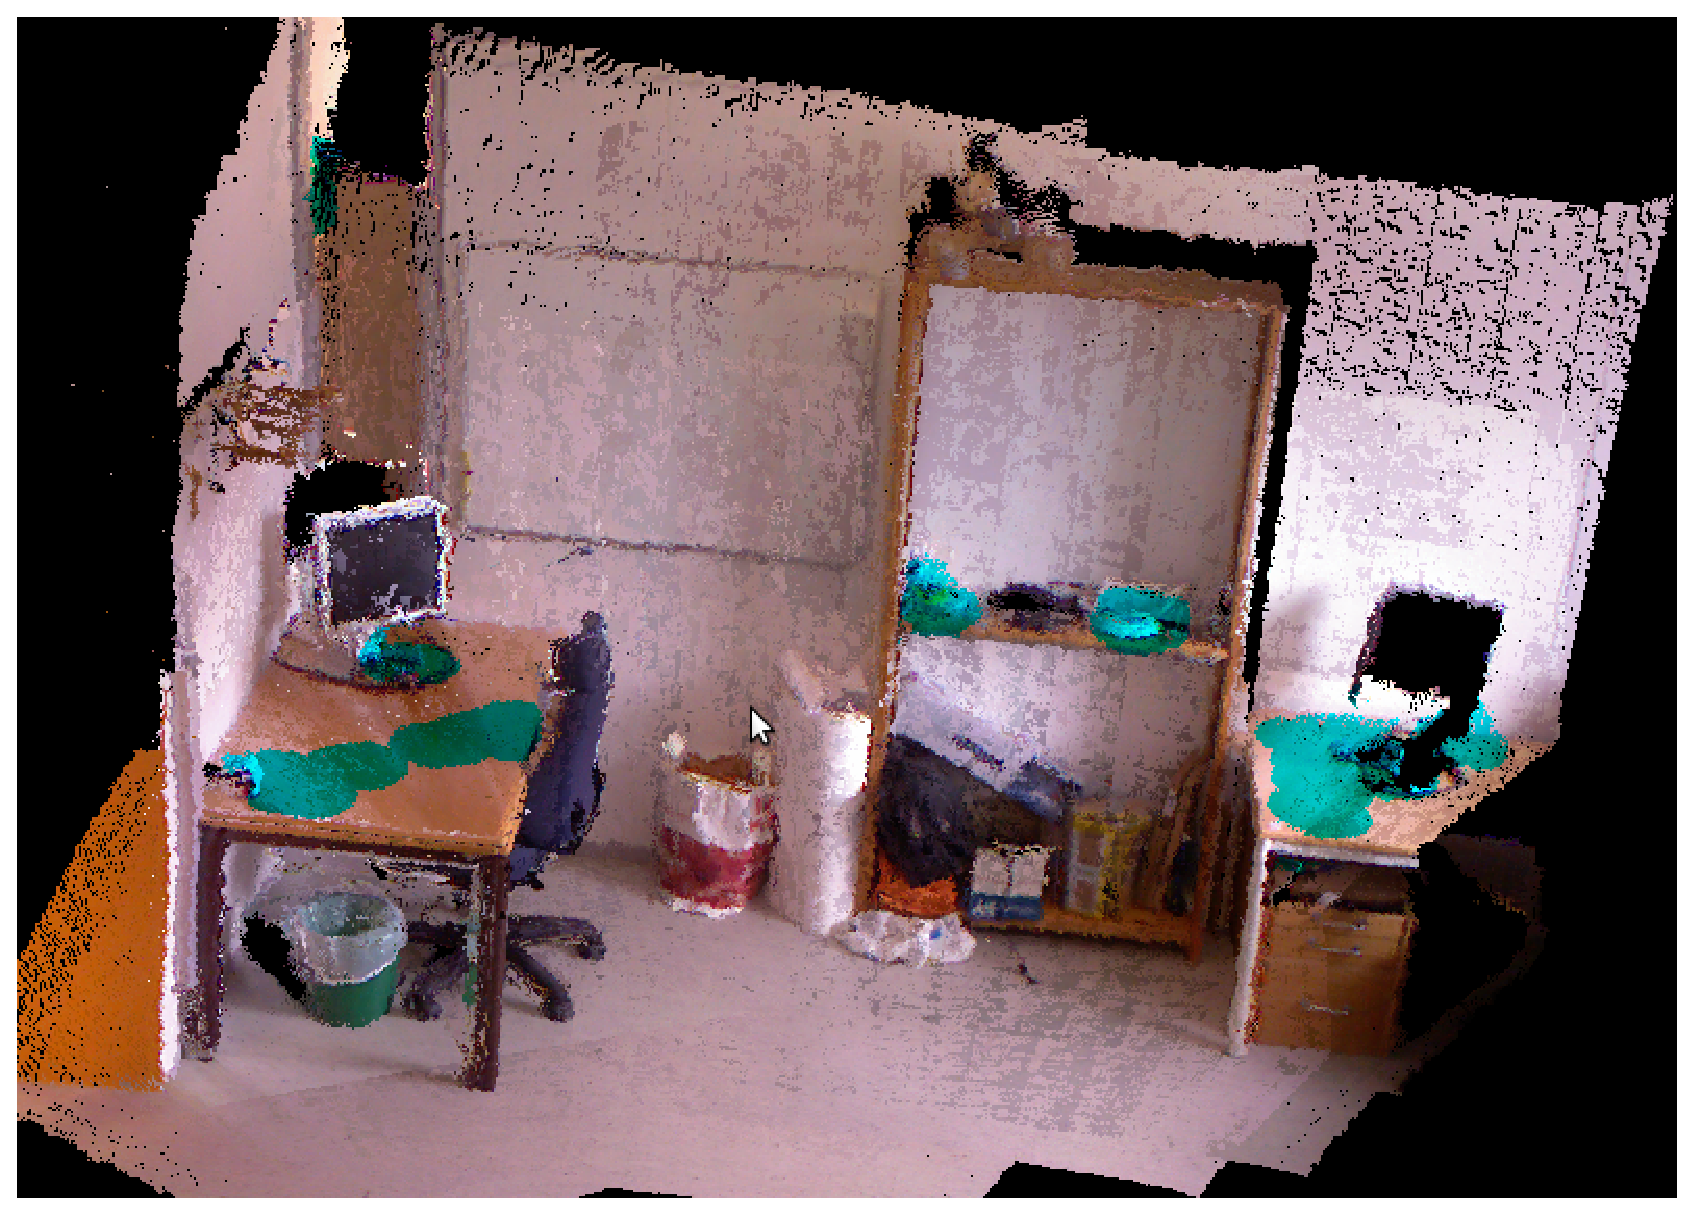
\includegraphics[width=2in,height=2in]{./Figures/Test_telefonPredict_c10g0.eps}}
%     \subfigure[Predicted context for Trash Bin.]{\label{ContextPrediction_Test_512.figure:TrashBin}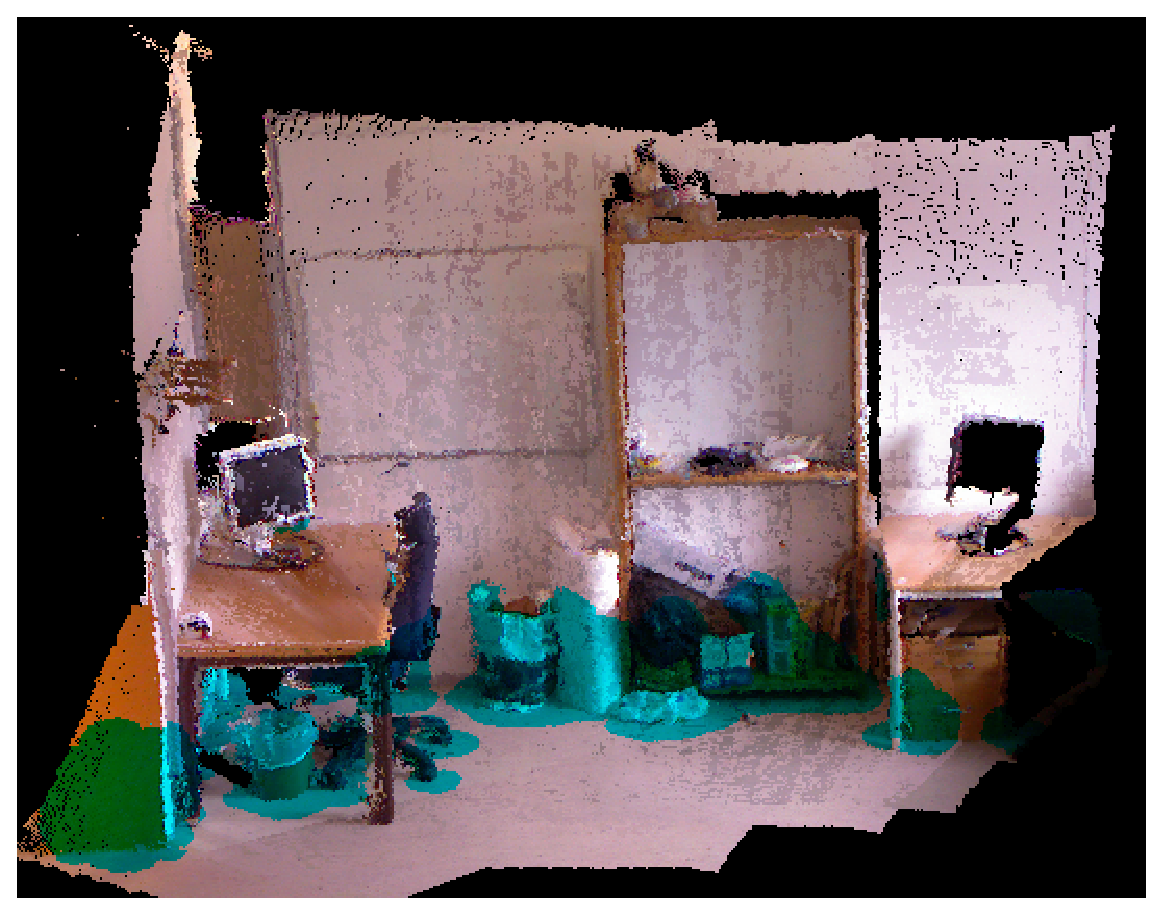
\includegraphics[width=2in,height=2in]{./Figures/Test_TrashBinPrediction_c1g0.eps}} \\
%   \end{center}
%   \caption[Visualization of context model prediction on sample cloud 2 as a test cloud.]
%   {Visualization of context model prediction on sample cloud 2 as a test cloud for four objects. This pointcloud does not include 
%   these objects except trash bin.(best viewed in color)}
%   \label{ContextPrediction_Test_512.figure:edge}
% \end{figure}
% 
% Figure ~\ref{ContextPrediction_Test_512.figure:edge} shows the predicted contexts of these four object class on the 
% pointcloud of an office from test set.
% In this test cloud no instance of wiper, mouse or telephone is present.
% The reasonability of the predicted object contexts are visible in this figure despite absence of those instances.
% 
% \subsection*{Summery}
% As mentioned in Section \ref{ExperimentalSetup.sec}, in the experiments we used pointclouds of different place categories like 
% kitchen, bathroom and offices which included a number of instances of the four object category.
% Each of these pointclouds in average contained around 8 million points out of which we extracted samples for a number of keypoints.
% The average number of samples extracted from each pointcloud is approximately 50000.
% Samples from several pointclouds are assembled in a set from which a train set is derived.
% The set of clouds are divided into train (45\%), validation (15\%) and test(40\%).
% Parameter and best model selection is done using validation set.
% 
% The results show that the predicted context is able to reduce the search space significantly while preserves the high chance of
% finding the object of interest.
% It also implies that the context of objects are modeled in a reliable way which makes it useful in place categorization where
% we need to know just the possibility of presence of an object class in a query place (discussed in Chapter \ref{UsingObjectContextforPlaceClassification.ch}).
% By tweaking the threshold of the prediction, the search space can be extended in a smart way rather than a greedy manner.
% 
% The time needed to train a model depends on the size of train set and the used parameters which in these experiments is in average
% 89 second.
% Test takes approximately 45 second and the time needed for feature extraction per sample is 68 ms.
% 
% 
% 
% \begin{figure}[t]
%   \centerpsw{Eval80Experiment}{0.65\columnwidth}
%   \caption[]
%   {}
%   \label{}
% \end{figure}
% 
% 
% \begin{figure}[t]
%   \centerpsw{log(w1w-1)}{0.65\columnwidth}
%   \caption[]
%   {}
%   \label{}
% \end{figure}
% 
% \begin{figure}[t]
%   \centerpsw{PositiveRatio}{0.65\columnwidth}
%   \caption[]
%   {}
%   \label{}
% \end{figure}
% 
% \begin{figure}[t]
%   \centerpsw{TruePositiveRatio}{0.65\columnwidth}
%   \caption[]
%   {}
%   \label{}
% \end{figure}
% 
% \begin{figure}[t]
%   \centerpsw{w1w-1}{0.65\columnwidth}
%   \caption[]
%   {}
%   \label{}
% \end{figure}
% 
% 
